\documentclass[10pt]{article}

% ── Packages ──────────────────────────────────────────────────────
\usepackage[top=0.85in,bottom=0.85in,left=0.9in,right=0.9in]{geometry}
\usepackage{amsmath,amssymb,amsthm}
\usepackage{bm}
\usepackage{booktabs}
\usepackage{graphicx}
\usepackage{enumitem}
\usepackage{hyperref}
\usepackage{cleveref}
\usepackage{caption}
\usepackage{subcaption}
\usepackage{float}
\usepackage{setspace}
\usepackage[numbers]{natbib}
\usepackage{titlesec}

% ── Line spacing: compact ─────────────────────────────────────────
\setstretch{1.02}
\setlength{\parskip}{0pt plus 0.5pt}

% ── Tighter float spacing ────────────────────────────────────────
\setlength{\textfloatsep}{8pt plus 2pt minus 2pt}
\setlength{\floatsep}{8pt plus 2pt minus 2pt}
\setlength{\intextsep}{6pt plus 2pt minus 2pt}
\setlength{\abovecaptionskip}{4pt}
\setlength{\belowcaptionskip}{2pt}

% ── Smaller section titles ───────────────────────────────────────
\titleformat{\section}{\normalsize\bfseries}{\thesection}{1em}{}
\titleformat{\subsection}{\small\bfseries}{\thesubsection}{1em}{}
\titleformat{\subsubsection}{\small\itshape}{\thesubsubsection}{1em}{}
\titlespacing*{\section}{0pt}{1.0ex plus .3ex minus .2ex}{0.4ex plus .1ex}
\titlespacing*{\subsection}{0pt}{0.8ex plus .2ex minus .2ex}{0.3ex plus .1ex}
\titlespacing*{\subsubsection}{0pt}{0.6ex plus .2ex minus .1ex}{0.2ex plus .1ex}

% ── Tighter math spacing ─────────────────────────────────────────
\setlength{\abovedisplayskip}{4pt plus 2pt minus 2pt}
\setlength{\belowdisplayskip}{4pt plus 2pt minus 2pt}
\setlength{\abovedisplayshortskip}{2pt plus 1pt}
\setlength{\belowdisplayshortskip}{2pt plus 1pt}

% ── Tighter list spacing ────────────────────────────────────────
\setlist{topsep=2pt, itemsep=1pt, parsep=0pt}

% ── Figure path ───────────────────────────────────────────────────
\graphicspath{{../output/figures/}}

% ── Shortcuts ─────────────────────────────────────────────────────
\newcommand{\bx}{\bm{x}}
\newcommand{\bX}{\bm{X}}
\newcommand{\by}{\bm{y}}
\newcommand{\bbeta}{\bm{\beta}}
\newcommand{\bu}{\bm{u}}
\newcommand{\btheta}{\bm{\theta}}
\newcommand{\iid}{\overset{\text{iid}}{\sim}}
\newcommand{\ind}{\overset{\text{ind}}{\sim}}
\DeclareMathOperator{\logit}{logit}
\DeclareMathOperator{\Bernoulli}{Bernoulli}
\DeclareMathOperator{\Normal}{\mathcal{N}}
\DeclareMathOperator{\HalfNormal}{Half\text{-}Normal}
\DeclareMathOperator{\HalfCauchy}{Half\text{-}Cauchy}

\newtheorem{proposition}{Proposition}
\newtheorem{remark}{Remark}

% ══════════════════════════════════════════════════════════════════
\title{\textbf{Bayesian Hierarchical Logistic Regression for\\
       30-Day Hospital Readmission Among Diabetic Patients:\\
       The Role of Medical Specialty}}
\author{Xingyu You \and Zhouhan Qian}
\date{April 2026}

\begin{document}
\maketitle

\begin{abstract}
Hospital readmission within 30 days is a costly and clinically important outcome. We investigate whether medical specialty contributes to readmission risk after adjusting for patient characteristics using a Bayesian hierarchical logistic regression with specialty-specific random intercepts, fitted via a custom Metropolis-within-Gibbs sampler on 37{,}964 diabetic encounters across 19 specialties. Substantial between-specialty heterogeneity is observed ($\hat{\tau} = 0.437$, 95\% CrI $[0.298, 0.644]$), with Physical Medicine and Rehabilitation exhibiting markedly elevated risk. Key predictors include prior inpatient visits (OR $= 1.22$), comorbid neoplasms (OR $= 1.51$), and A1C measurement (OR $= 1.42$). Results are robust to prior sensitivity analysis.
\end{abstract}

% ══════════════════════════════════════════════════════════════════
\section{Introduction}
% ══════════════════════════════════════════════════════════════════

Unplanned hospital readmissions within 30 days of discharge represent a major burden on healthcare systems, with annual costs exceeding \$26 billion in the United States. Patients with diabetes, characterised by high comorbidity and complex medication regimens, experience particularly high readmission rates. The Centers for Medicare \& Medicaid Services (CMS) has introduced financial penalties for hospitals with excess readmissions, making reduction efforts both clinically and economically important.

Previous studies have identified patient-level predictors of readmission, such as length of stay, prior admissions, and comorbidity burden, typically using logistic regression or machine learning models. However, an important structural factor is often overlooked: patients are managed by physicians from different medical specialties, which may vary in post-discharge care patterns, case mix, and practice style. Ignoring this clustering can violate independence assumptions, bias standard errors, and obscure opportunities for specialty-level intervention.

This study examines whether specialty-level heterogeneity contributes to 30-day readmission risk among diabetic patients after adjusting for patient-level covariates. The analysis is complicated by substantial group-size imbalance, with some specialties contributing large numbers of encounters while others have relatively few, making naïve comparisons unreliable due to sampling variability.

A Bayesian hierarchical model is well suited to this setting. Partial pooling allows small-sample specialties to borrow strength from larger groups through the shared hyperparameter $\tau$, yielding more stable estimates than complete or no pooling. The Bayesian framework provides coherent uncertainty quantification via posterior credible intervals for $\tau$, directly characterising between-specialty variation without reliance on $p$-values. Model assessment can be conducted using DIC and posterior predictive checks within a unified framework. In addition, the hierarchical prior induces shrinkage on random intercepts, acting as adaptive regularisation and controlling model complexity without requiring cross-validation.

% ══════════════════════════════════════════════════════════════════
\section{Data and Cohort Definition}
% ══════════════════════════════════════════════════════════════════

\subsection{Data Source}

We use the Diabetes 130-US Hospitals dataset \citep{strack2014diabetes}, comprising 101{,}766 inpatient encounters from 130 US hospitals over 1999-2008, with detailed demographic, clinical, and medication information.

\subsection{Cohort Construction}

Starting from $N_{\text{raw}} = 101{,}766$, variables with high missingness or no variation were removed, including weight, payer\_code, citoglipton, and examide. To ensure independence, only the first encounter per patient was retained, yielding $N = 71{,}518$. Encounters corresponding to expired or hospice discharges were excluded, leaving $N = 69{,}973$. The outcome was defined as $y_i = 1$ for readmission within 30 days ($<30$), and $0$ otherwise. Encounters with unknown specialty were excluded (45.7\%), resulting in $N = 37{,}965$, and specialties were grouped into $J = 19$ categories by merging small groups. One record with unknown gender was removed, yielding a final sample size of $N = 37{,}964$. Continuous variables were standardised to $z$-scores, and categorical features were constructed from demographics, ICD-9 diagnosis groups, comorbidities, and medication indicators. The final dataset includes $N = 37{,}964$ encounters, $J = 19$ specialties, $K = 43$ covariates, and a 30-day readmission rate of $9.60\%$.

The cohort has a mean age of 64.9 years, with $53.5\%$ female and $73.0\%$ Caucasian patients. Readmitted patients are older and exhibit greater clinical complexity, including longer stays, more medications, more prior inpatient visits, and more diagnoses.

Specialty group sizes range from 288 (Physical Medicine and Rehabilitation) to
10,975 (Internal Medicine), with raw readmission rates spanning 4.3\%
(Obstetrics/Gynecology) to 32.3\% (Physical Medicine and Rehabilitation).
The wide dispersion in unadjusted readmission rates motivates a model that accounts for specialty-level heterogeneity.

% ══════════════════════════════════════════════════════════════════
\section{Model Specification}
\label{sec:model}
% ══════════════════════════════════════════════════════════════════

\subsection{Notation}

\begin{table}[H]
\centering
\small
\caption{Summary of notation.}
\label{tab:notation}
\begin{tabular}{cl}
\toprule
Symbol & Meaning \\
\midrule
$N = 37{,}964$ & Number of observations (encounters) \\
$K = 43$        & Number of patient-level covariates \\
$J = 19$        & Number of medical specialty groups \\
$y_i \in \{0,1\}$ & 30-day readmission indicator for encounter $i$ \\
$\bx_i \in \mathbb{R}^K$ & Covariate vector for encounter $i$ \\
$j[i] \in \{1,\dots,J\}$ & Specialty group index for encounter $i$ \\
$n_j$ & Number of observations in group $j$ \\
$\alpha \in \mathbb{R}$ & Global intercept \\
$\bbeta \in \mathbb{R}^K$ & Fixed-effect coefficients \\
$u_j \in \mathbb{R}$ & Random intercept for specialty group $j$ \\
$\bu = (u_1,\dots,u_J)^\top$ & Vector of all random intercepts \\
$\tau > 0$ & Between-group standard deviation \\
$\eta_i$ & Linear predictor for observation $i$ \\
\bottomrule
\end{tabular}
\end{table}

\subsection{Likelihood}

For encounter $i$, the model decomposes the log-odds of readmission into
three additive pieces: a global baseline $\alpha$, a patient-level term
$\bx_i^\top \bbeta$, and a specialty-specific deviation $u_{j[i]}$.
Conditional on these quantities, the observed outcome is Bernoulli:
\begin{equation}
  y_i \mid \alpha, \bbeta, \bu \;\ind\;
  \Bernoulli(\pi_i), \quad
  \pi_i = \frac{\exp(\eta_i)}{1 + \exp(\eta_i)}, \quad
  \eta_i = \alpha + \bx_i^\top \bbeta + u_{j[i]},
\end{equation}
where $\bx_i \in \mathbb{R}^{K}$ is the engineered covariate vector
($K = 43$), $j[i] \in \{1,\dots,J\}$ identifies the specialty group, and
$u_{j[i]}$ is that group's random intercept.  In the implementation,
continuous covariates are standardised, race and primary-diagnosis group
enter through reference-category indicators, and binary or ordinal clinical
features are included directly in $\bx_i$.

The full likelihood is:
\begin{equation}
  p(\by \mid \alpha, \bbeta, \bu)
  = \prod_{i=1}^{N} \frac{\exp(y_i\,\eta_i)}{1 + \exp(\eta_i)}.
\end{equation}

\subsection{Prior Distributions}

\begin{align}
  \alpha &\sim \Normal(0, \sigma_\alpha^2), && \sigma_\alpha = 5, \\
  \beta_k &\iid \Normal(0, s_\beta^2), && s_\beta = 2.5, \quad k = 1,\dots,K, \\
  u_j \mid \tau &\iid \Normal(0, \tau^2), && j = 1,\dots,J, \\
  \tau &\sim \HalfNormal(0, s_\tau^2), && s_\tau = 1.0.
\end{align}
The Half-Normal density is
$p(\tau) = \frac{2}{\sqrt{2\pi}\,s_\tau}\exp\!\bigl(-\tfrac{\tau^2}{2s_\tau^2}\bigr)$
for $\tau > 0$.
As a sensitivity alternative (Section~\ref{sec:sensitivity}), we also consider
$\tau \sim \HalfCauchy(0,\,s_\tau)$ with density
$p(\tau) = \frac{2}{\pi\,s_\tau}\,\frac{1}{1 + \tau^2/s_\tau^2}$, $\tau > 0$.

The priors are weakly informative \citep{gelman2013bda}, chosen to impose
minimal substantive constraint while ensuring posterior propriety. The
intercept prior with $\sigma_\alpha = 5$ places nearly all mass on baseline
probabilities ranging from approximately $0.005\%$ to $99.995\%$, far wider
than any clinically plausible readmission rate. The fixed-effect prior with
$s_\beta = 2.5$ allows odds ratios as large as $e^5 \approx 150$, so it is
effectively non-informative for well-identified coefficients while still
providing mild regularisation for weaker ones. For the group-level scale, the
$\HalfNormal(0,1)$ prior concentrates mass near zero while permitting
substantial heterogeneity \citep{gelman2006prior}; on the log-odds scale,
$\tau = 1$ corresponds to roughly 2.7-fold variation in odds between
specialties at $\pm 1$~SD, which is already large.

\subsection{Hierarchical Interpretation}

The hierarchical component of the model is the prior
$u_j \mid \tau \iid \Normal(0, \tau^2)$.  The $u_j$'s are latent
specialty effects: they are not observed directly, but inferred jointly with
the rest of the parameters.  Conditional on $\tau$, these effects are
exchangeable, meaning that before seeing the data we treat specialties as
coming from a common population centered at zero.

The scale parameter $\tau$ controls how strongly the model pools information
across specialties.  When $\tau$ is small, the prior strongly pulls all
specialty effects toward zero, so the model behaves close to a common-intercept
logistic regression.  When $\tau$ is large, specialties are allowed to differ
more freely, approaching a no-pooling analysis with separate intercepts.

For intuition, it is helpful to think of the posterior estimate of $u_j$ as a
compromise between the within-specialty signal and the prior pull toward zero.
This is not an exact closed-form result for the logistic model, but a useful
normal-approximation heuristic is:
\begin{equation}\label{eq:shrinkage}
  \hat{u}_j^{\text{Bayes}} \;\approx\;
  \underbrace{\frac{n_j / \hat{\sigma}_j^2}{n_j / \hat{\sigma}_j^2 + 1/\hat{\tau}^2}}_{\text{shrinkage weight } \lambda_j}
  \;\hat{u}_j^{\text{MLE}},
\end{equation}
where $\hat{\sigma}_j^2$ is the within-group variance of the linear predictor
residuals.  The shrinkage weight $\lambda_j \in [0,1]$ depends on the
signal-to-noise ratio within each group. As $\tau \to 0$, $\lambda_j \to 0$
for all $j$, so all specialties collapse to a common intercept; as
$\tau \to \infty$, $\lambda_j \to 1$, recovering a no-pooling analysis with
group-specific intercepts. For intermediate $\tau$, which is the empirically
relevant case here, large groups such as Internal Medicine ($n = 10{,}975$)
have $\lambda_j \approx 1$ and are barely shrunk, whereas smaller groups such
as PMR ($n = 288$) have noticeably smaller $\lambda_j$ and are pulled toward
the grand mean. This adaptive, data-driven regularisation is the core
advantage of the hierarchical approach.

\subsection{Assumptions and Encoding}

The model assumes conditional independence of outcomes given the parameters,
uses only the first encounter per patient, treats specialty assignment as
exogenous, and includes specialty-specific random intercepts but no random
slopes. Continuous predictors are standardised to mean zero and variance one to
stabilise computation and make coefficients comparable across scales. Race and
primary-diagnosis group are encoded through reference-category indicators
(reference levels: Caucasian and Circulatory, respectively), whereas
\texttt{A1C\_level} and \texttt{glu\_level} enter as ordinal covariates. A
priori, $\alpha$, $\bbeta$, and $\tau$ are independent, and $\bu$ depends on
$\tau$ only through the hierarchical prior.

\subsection{Hyperparameters}

\begin{table}[H]
\centering
\caption{Hyperparameter settings and their interpretation.}
\label{tab:hyperparams}
\begin{tabular}{cll}
\toprule
Symbol & Value & Role \\
\midrule
$\sigma_\alpha$ & 5.0 & Prior SD for the intercept; covers plausible baseline log-odds \\
$s_\beta$ & 2.5 & Prior SD for each fixed effect; allows OR up to $\sim e^{5} \approx 150$ \\
$s_\tau$ & 1.0 & Scale of the half-normal hyperprior on $\tau$; concentrates mass near zero \\
\bottomrule
\end{tabular}
\end{table}

% ══════════════════════════════════════════════════════════════════
\section{Posterior Derivation}
\label{sec:derivation}
% ══════════════════════════════════════════════════════════════════

\subsection{Joint Distribution}

By the conditional independence structure of the hierarchical model,
the joint distribution of all observables and parameters factorises as:
\begin{equation}\label{eq:joint}
  p(\by,\alpha,\bbeta,\bu,\tau \mid \bX)
  = \underbrace{p(\by \mid \alpha,\bbeta,\bu,\bX)}_{\text{likelihood}}
    \;\underbrace{p(\alpha)}_{\text{prior on }\alpha}
    \;\underbrace{p(\bbeta)}_{\text{prior on }\bbeta}
    \;\underbrace{p(\bu \mid \tau)}_{\text{random effects}}
    \;\underbrace{p(\tau)}_{\text{hyperprior}}.
\end{equation}
Substituting each component explicitly:
\begin{align}
  p(\by,\alpha,\bbeta,\bu,\tau \mid \bX)
  &= \prod_{i=1}^{N}\frac{\exp(y_i\,\eta_i)}{1+\exp(\eta_i)}
  \;\cdot\;
  \frac{1}{\sqrt{2\pi}\,\sigma_\alpha}
  \exp\!\Bigl(-\frac{\alpha^2}{2\sigma_\alpha^2}\Bigr)
  \notag\\
  &\quad\;\cdot\;
  \prod_{k=1}^{K}\frac{1}{\sqrt{2\pi}\,s_\beta}
  \exp\!\Bigl(-\frac{\beta_k^2}{2s_\beta^2}\Bigr)
  \;\cdot\;
  \prod_{j=1}^{J}\frac{1}{\sqrt{2\pi}\,\tau}
  \exp\!\Bigl(-\frac{u_j^2}{2\tau^2}\Bigr)
  \notag\\
  &\quad\;\cdot\;
  \frac{2}{\sqrt{2\pi}\,s_\tau}
  \exp\!\Bigl(-\frac{\tau^2}{2s_\tau^2}\Bigr)
  \;\mathbf{1}(\tau > 0).
  \label{eq:joint-full}
\end{align}

\subsection{Posterior Distribution (Up to Proportionality)}

By Bayes' theorem, the posterior is proportional to the joint:
\begin{equation}\label{eq:posterior}
  p(\alpha,\bbeta,\bu,\tau \mid \by, \bX)
  = \frac{p(\by,\alpha,\bbeta,\bu,\tau \mid \bX)}{p(\by \mid \bX)}
  \;\propto\;
  p(\by \mid \alpha,\bbeta,\bu,\bX)\;
  p(\alpha)\;p(\bbeta)\;p(\bu\mid\tau)\;p(\tau),
\end{equation}
where the marginal likelihood $p(\by \mid \bX) = \int p(\by,\alpha,\bbeta,\bu,\tau \mid \bX)\,d\alpha\,d\bbeta\,d\bu\,d\tau$ is an intractable normalising constant.

\subsection{Log-Posterior}

Taking logarithms of~\eqref{eq:joint-full} and dropping additive constants
that do not depend on any parameter:
\begin{align}
  \ell(\alpha,\bbeta,\bu,\tau)
  &\;=\; \log p(\alpha,\bbeta,\bu,\tau \mid \by,\bX) + \text{const.} \notag\\
  &\;=\;
  \underbrace{\sum_{i=1}^{N}
    \bigl[y_i\,\eta_i - \log(1+e^{\eta_i})\bigr]}_{\text{(I) log-likelihood}}
  \;-\;
  \underbrace{\frac{\alpha^2}{2\sigma_\alpha^2}}_{\text{(II) prior on }\alpha}
  \;-\;
  \underbrace{\frac{1}{2s_\beta^2}\sum_{k=1}^{K}\beta_k^2}_{\text{(III) prior on }\bbeta}
  \notag\\
  &\quad\;-\;
  \underbrace{J\log\tau \;+\;
  \frac{1}{2\tau^2}\sum_{j=1}^{J}u_j^2}_{\text{(IV) }p(\bu\mid\tau)}
  \;-\;
  \underbrace{\frac{\tau^2}{2s_\tau^2}}_{\text{(V) hyperprior on }\tau}.
  \label{eq:logpost}
\end{align}

\begin{remark}
The log-likelihood term uses the identity
$\log\bigl(\pi_i^{y_i}(1-\pi_i)^{1-y_i}\bigr) = y_i\eta_i - \log(1+e^{\eta_i})$,
which avoids computing $\pi_i$ explicitly and is numerically stable
when implemented as $\log(1+e^{\eta_i}) = \mathrm{logaddexp}(0,\eta_i)$.
\end{remark}

The logistic likelihood makes this posterior non-conjugate, so none of the
parameter blocks has a closed-form Gibbs update.  Instead, for each block we
write down the log-target up to an additive constant and use that target in a
Metropolis step.

\subsection{Block-Specific Log-Targets}

For a given parameter block, the relevant target is obtained by collecting the
terms in~\eqref{eq:logpost} that depend on that block and treating everything
else as constant. Because the sampler uses symmetric random-walk proposals, the
Hastings correction cancels and each acceptance ratio takes the form
$\log R = h(\theta^*) - h(\theta^{(t)})$.

As a representative example, the intercept appears in every observation
through $\eta_i = \alpha + \bx_i^\top\bbeta + u_{j[i]}$, so its log-target is
\begin{equation}\label{eq:fc-alpha}
  h(\alpha) = \sum_{i=1}^{N}
    \bigl[y_i\,\eta_i - \log(1+e^{\eta_i})\bigr]
  - \frac{\alpha^2}{2\sigma_\alpha^2}.
\end{equation}
This combines the full likelihood with the Gaussian prior penalty. The
fixed-effect updates are analogous, replacing the intercept penalty by
$-\beta_k^2/(2s_\beta^2)$ and modifying the linear predictor only through the
single column $x_{ik}$. For each random intercept $u_j$, the likelihood sum is
restricted to observations in specialty $j$ and the prior contribution becomes
$-u_j^2/(2\tau^2)$, reducing the update cost from $O(N)$ to $O(n_j)$.

For the scale parameter we work on the unconstrained scale $\phi = \log\tau$.
Substituting $\tau = e^\phi$ into~\eqref{eq:logpost} and adding the Jacobian
term $\phi$ yields
\begin{equation}
  h(\phi)
  = -J\,\phi
    - \frac{1}{2e^{2\phi}}\sum_{j=1}^{J}u_j^2
    - \frac{e^{2\phi}}{2s_\tau^2}
    + \phi
  = -(J-1)\,\phi
     - \frac{1}{2e^{2\phi}}\sum_{j=1}^{J}u_j^2
     - \frac{e^{2\phi}}{2s_\tau^2}.
  \label{eq:fc-log-tau}
\end{equation}
Conditional on $\bu$, the likelihood does not depend on $\tau$ directly, so
this update costs only $O(J)$. Under the sensitivity prior
$\tau \sim \HalfCauchy(0, s_\tau)$, the last term in~\eqref{eq:fc-log-tau} is
replaced by the heavier-tailed penalty
\begin{equation}\label{eq:fc-log-tau-hc}
  h_{\text{HC}}(\phi)
  = -(J-1)\,\phi
    - \frac{1}{2e^{2\phi}}\sum_{j=1}^{J}u_j^2
    - \log\!\Bigl(1 + \frac{e^{2\phi}}{s_\tau^2}\Bigr).
\end{equation}

\subsection{Posterior Propriety}

\begin{proposition}
Under the model specified in Section~\ref{sec:model}, the posterior
$p(\alpha,\bbeta,\bu,\tau \mid \by,\bX)$ is proper (i.e., integrable).
\end{proposition}
\begin{proof}
We verify integrability of each factor in the joint~\eqref{eq:joint-full}:
\begin{enumerate}[label=(\alph*)]
  \item \textbf{Likelihood.} For any fixed $(\alpha,\bbeta,\bu)$, the
    Bernoulli likelihood satisfies $0 \le p(\by \mid \alpha,\bbeta,\bu) \le 1$.
  \item \textbf{Prior on $\alpha$.} $\alpha \sim \Normal(0, \sigma_\alpha^2)$
    is proper, so $\int p(\alpha)\,d\alpha = 1$.
  \item \textbf{Prior on $\bbeta$.} Each $\beta_k \sim \Normal(0, s_\beta^2)$
    independently; the product of $K$ proper Gaussians is proper.
  \item \textbf{Conditional prior $p(\bu \mid \tau)$.} For any fixed $\tau > 0$,
    each $u_j \sim \Normal(0,\tau^2)$ is proper.
  \item \textbf{Hyperprior on $\tau$.} $\HalfNormal(0, s_\tau^2)$ is proper on $(0,\infty)$.
\end{enumerate}
Therefore:
\[
  \int p(\by \mid \cdot)\,p(\alpha)\,p(\bbeta)\,p(\bu\mid\tau)\,p(\tau)
  \;d\alpha\,d\bbeta\,d\bu\,d\tau
  \;\le\;
  \underbrace{\int p(\alpha)\,d\alpha}_{=1}\;
  \underbrace{\int p(\bbeta)\,d\bbeta}_{=1}\;
  \int p(\tau)\underbrace{\int p(\bu\mid\tau)\,d\bu}_{=1}\,d\tau
  = 1 < \infty.
\]
Since all priors are proper and the likelihood is bounded, the marginal likelihood is finite and the posterior is proper.
\end{proof}

\subsection{Identifiability}

\paragraph{Weak non-identifiability of $\alpha$ and $\bu$.}
If we define $\alpha' = \alpha + c$ and $u_j' = u_j - c$ for any constant $c$, then
$\eta_i' = \alpha' + \bx_i^\top\bbeta + u_{j[i]}' = (\alpha + c) + \bx_i^\top\bbeta + (u_{j[i]} - c) = \eta_i$.
The likelihood alone cannot separate $\alpha$ from the mean of $\bu$.  In the Bayesian framework, this is resolved by the priors:
$p(\alpha) = \Normal(0,\sigma_\alpha^2)$ anchors $\alpha$ near zero, and
$p(u_j \mid \tau) = \Normal(0,\tau^2)$ centres each $u_j$ at zero.
Together these priors break the translation invariance.  Nevertheless, the posterior correlation between $\alpha$ and $\bar{u} = J^{-1}\sum_j u_j$ can be high, motivating the dedicated joint translation move (Block~5 in Section~\ref{sec:computation}).

\paragraph{Fixed effects.}
All continuous covariates are standardised (zero mean, unit variance),
which prevents collinearity between the intercept and covariate means.
Race and primary-diagnosis group use reference-category coding, while binary
indicators and ordinal lab summaries enter directly, yielding a full-rank
design matrix in the implemented feature set.

% ══════════════════════════════════════════════════════════════════
\section{Computational Strategy}
\label{sec:computation}
% ══════════════════════════════════════════════════════════════════

\subsection{Metropolis-within-Gibbs Sampler}

The logistic likelihood is non-conjugate, so standard Gibbs sampling is not
available, whereas full-dimensional Metropolis--Hastings on the
$(1 + K + J + 1) = 64$-dimensional parameter space would mix poorly. We
therefore use a random-walk \textbf{Metropolis-within-Gibbs (MwG)} sampler
based on the block-specific targets from Section~\ref{sec:derivation}. With
symmetric proposals $\theta^* = \theta^{(t)} + \epsilon$ and
$\epsilon \sim \Normal(0, \sigma_{\text{prop}}^2)$, the Hastings correction
cancels and the acceptance ratio reduces to
\begin{equation}\label{eq:log-ratio}
  \log R = h(\theta^*) - h(\theta^{(t)}).
\end{equation}

One MwG iteration updates $\alpha$, then $\beta_1,\dots,\beta_K$, then
$u_1,\dots,u_J$, then $\phi = \log\tau$, followed by $R = 10$ joint
translation moves of $(\alpha,\bu)$. The $\alpha$ update shifts all
$\eta_i$ by a constant and costs $O(N)$, each $\beta_k$ update costs $O(N)$,
each $u_j$ update costs $O(n_j)$, and the $\phi$ update costs $O(J)$ because
it involves no likelihood evaluation. Conditioning each step on the most
recently updated values defines a valid MwG chain whose stationary
distribution is the posterior~\eqref{eq:posterior}.

The most important nonstandard step is the joint translation move. Because the
transformation $\alpha \mapsto \alpha + c$ and $u_j \mapsto u_j - c$ leaves
all linear predictors unchanged, separate updates of $\alpha$ and $\bu$
explore this weakly identified ridge slowly. We therefore repeat the following
proposal $R = 10$ times per iteration: draw
$\delta \sim \Normal(0, \sigma_{\text{blk}}^2)$, set
$\alpha^* = \alpha + \delta$ and $u_j^* = u_j - \delta$ for all $j$, and
accept according to the prior-only ratio
\begin{equation}\label{eq:block5-ratio}
  \log R
  = \underbrace{-\frac{{\alpha^*}^2 - \alpha^2}{2\sigma_\alpha^2}}_{\text{intercept prior}}
  \;+\; \underbrace{\left(-\frac{\sum_j {u_j^*}^2 - \sum_j u_j^2}{2\tau^2}\right)}_{\text{random effect prior}}.
\end{equation}
This $O(J)$ move substantially improves mixing of the $\alpha$--$\bu$ block.

\subsection{Proposal Tuning}

Choosing appropriate proposal standard deviations $\sigma_{\text{prop}}$ is
critical: too small yields high acceptance but slow exploration; too large
yields low acceptance and wasted computation.  We tune each proposal SD
automatically using the pilot-tuning script in
\texttt{src/05b\_tune\_proposals.py}. Short pilot chains of 2,000 iterations
are run on a random subsample of $n = 20{,}000$ observations; after each
round, the empirical acceptance rate for each block is compared with the
target range $[0.20, 0.50]$, and the corresponding proposal SD is multiplied
by 1.5 if the rate is too high or by 0.5 if it is too low. Separate proposal
scales are maintained for each $\beta_k$ ($k = 1,\dots,43$) and each $u_j$
($j = 1,\dots,19$) to reflect differing posterior curvatures, and tuning stops
once all parameters, or at least 90\% of them, fall within the target range,
with a maximum of 20 pilot rounds.

For the present analysis, tuning stopped after 10 rounds. On the final pilot
round, the acceptance rates were $\alpha$: 0.40, $\bbeta$ (mean): 0.43,
$\bu$ (mean): 0.43, $\log\tau$: 0.37, and block move: 0.46, all within the
target range. In the subsequent full-data production run, the average
acceptance rates across the four chains were slightly lower
($\alpha$: 0.305, $\bbeta$: 0.331, $\bu$: 0.342, $\log\tau$: 0.372, block:
0.454), reflecting the sharper geometry of the full posterior.

\subsection{Chain Configuration}

We run four chains to diagnose convergence and reduce sensitivity to the
starting point.  The initial values are random but modest in scale:
$\alpha$ and $u_j$ are started near zero with Gaussian perturbations, the
$\beta_k$'s are initialised with small Gaussian noise, and $\tau$ is started
from a log-normal draw centered near 1. The production run used 4 chains of
30,000 iterations each, discarded the first 8,000 as burn-in, retained every
fifth draw, and therefore produced 4,400 post-burn-in samples per chain and
$4 \times 4{,}400 = 17{,}600$ pooled posterior draws; the random seed was 724.

The total computational cost is approximately $4 \times 30{,}000 \times
(1 + K + J + 1 + 10) = 4 \times 30{,}000 \times 74 \approx 8.9$ million
individual Metropolis steps.  Each step involves at most an $O(N)$ likelihood
evaluation.  According to the saved diagnostics, each chain required roughly
28--30 minutes, so four chains run sequentially complete in about two hours on
a single CPU core.

% ══════════════════════════════════════════════════════════════════
\section{Diagnostic Analysis}
\label{sec:diagnostics}
% ══════════════════════════════════════════════════════════════════

\subsection{Trace Plots and Autocorrelation}

Visual inspection of trace plots is a first-line diagnostic for MCMC
convergence.  For all parameters, we observe:
\begin{itemize}
  \item All four chains overlap and explore the same region of the parameter
    space, with no chain remaining isolated---evidence against multi-modality.
  \item No persistent trends or drifts after the burn-in period, suggesting
    the chains have reached stationarity.
  \item Autocorrelation functions decay rapidly to near zero within 20--50
    lags for most parameters, confirming that thinning by a factor of 5 is
    sufficient to produce approximately independent samples.
  \item The intercept $\alpha$ and the comorbidity-related coefficients (e.g.,
    $\beta_{28}$: comorbid\_circulatory, $\beta_{29}$:
    comorbid\_diabetes) show the highest autocorrelation, consistent
    with their posterior correlation structure.
\end{itemize}

\begin{figure}[H]
\centering
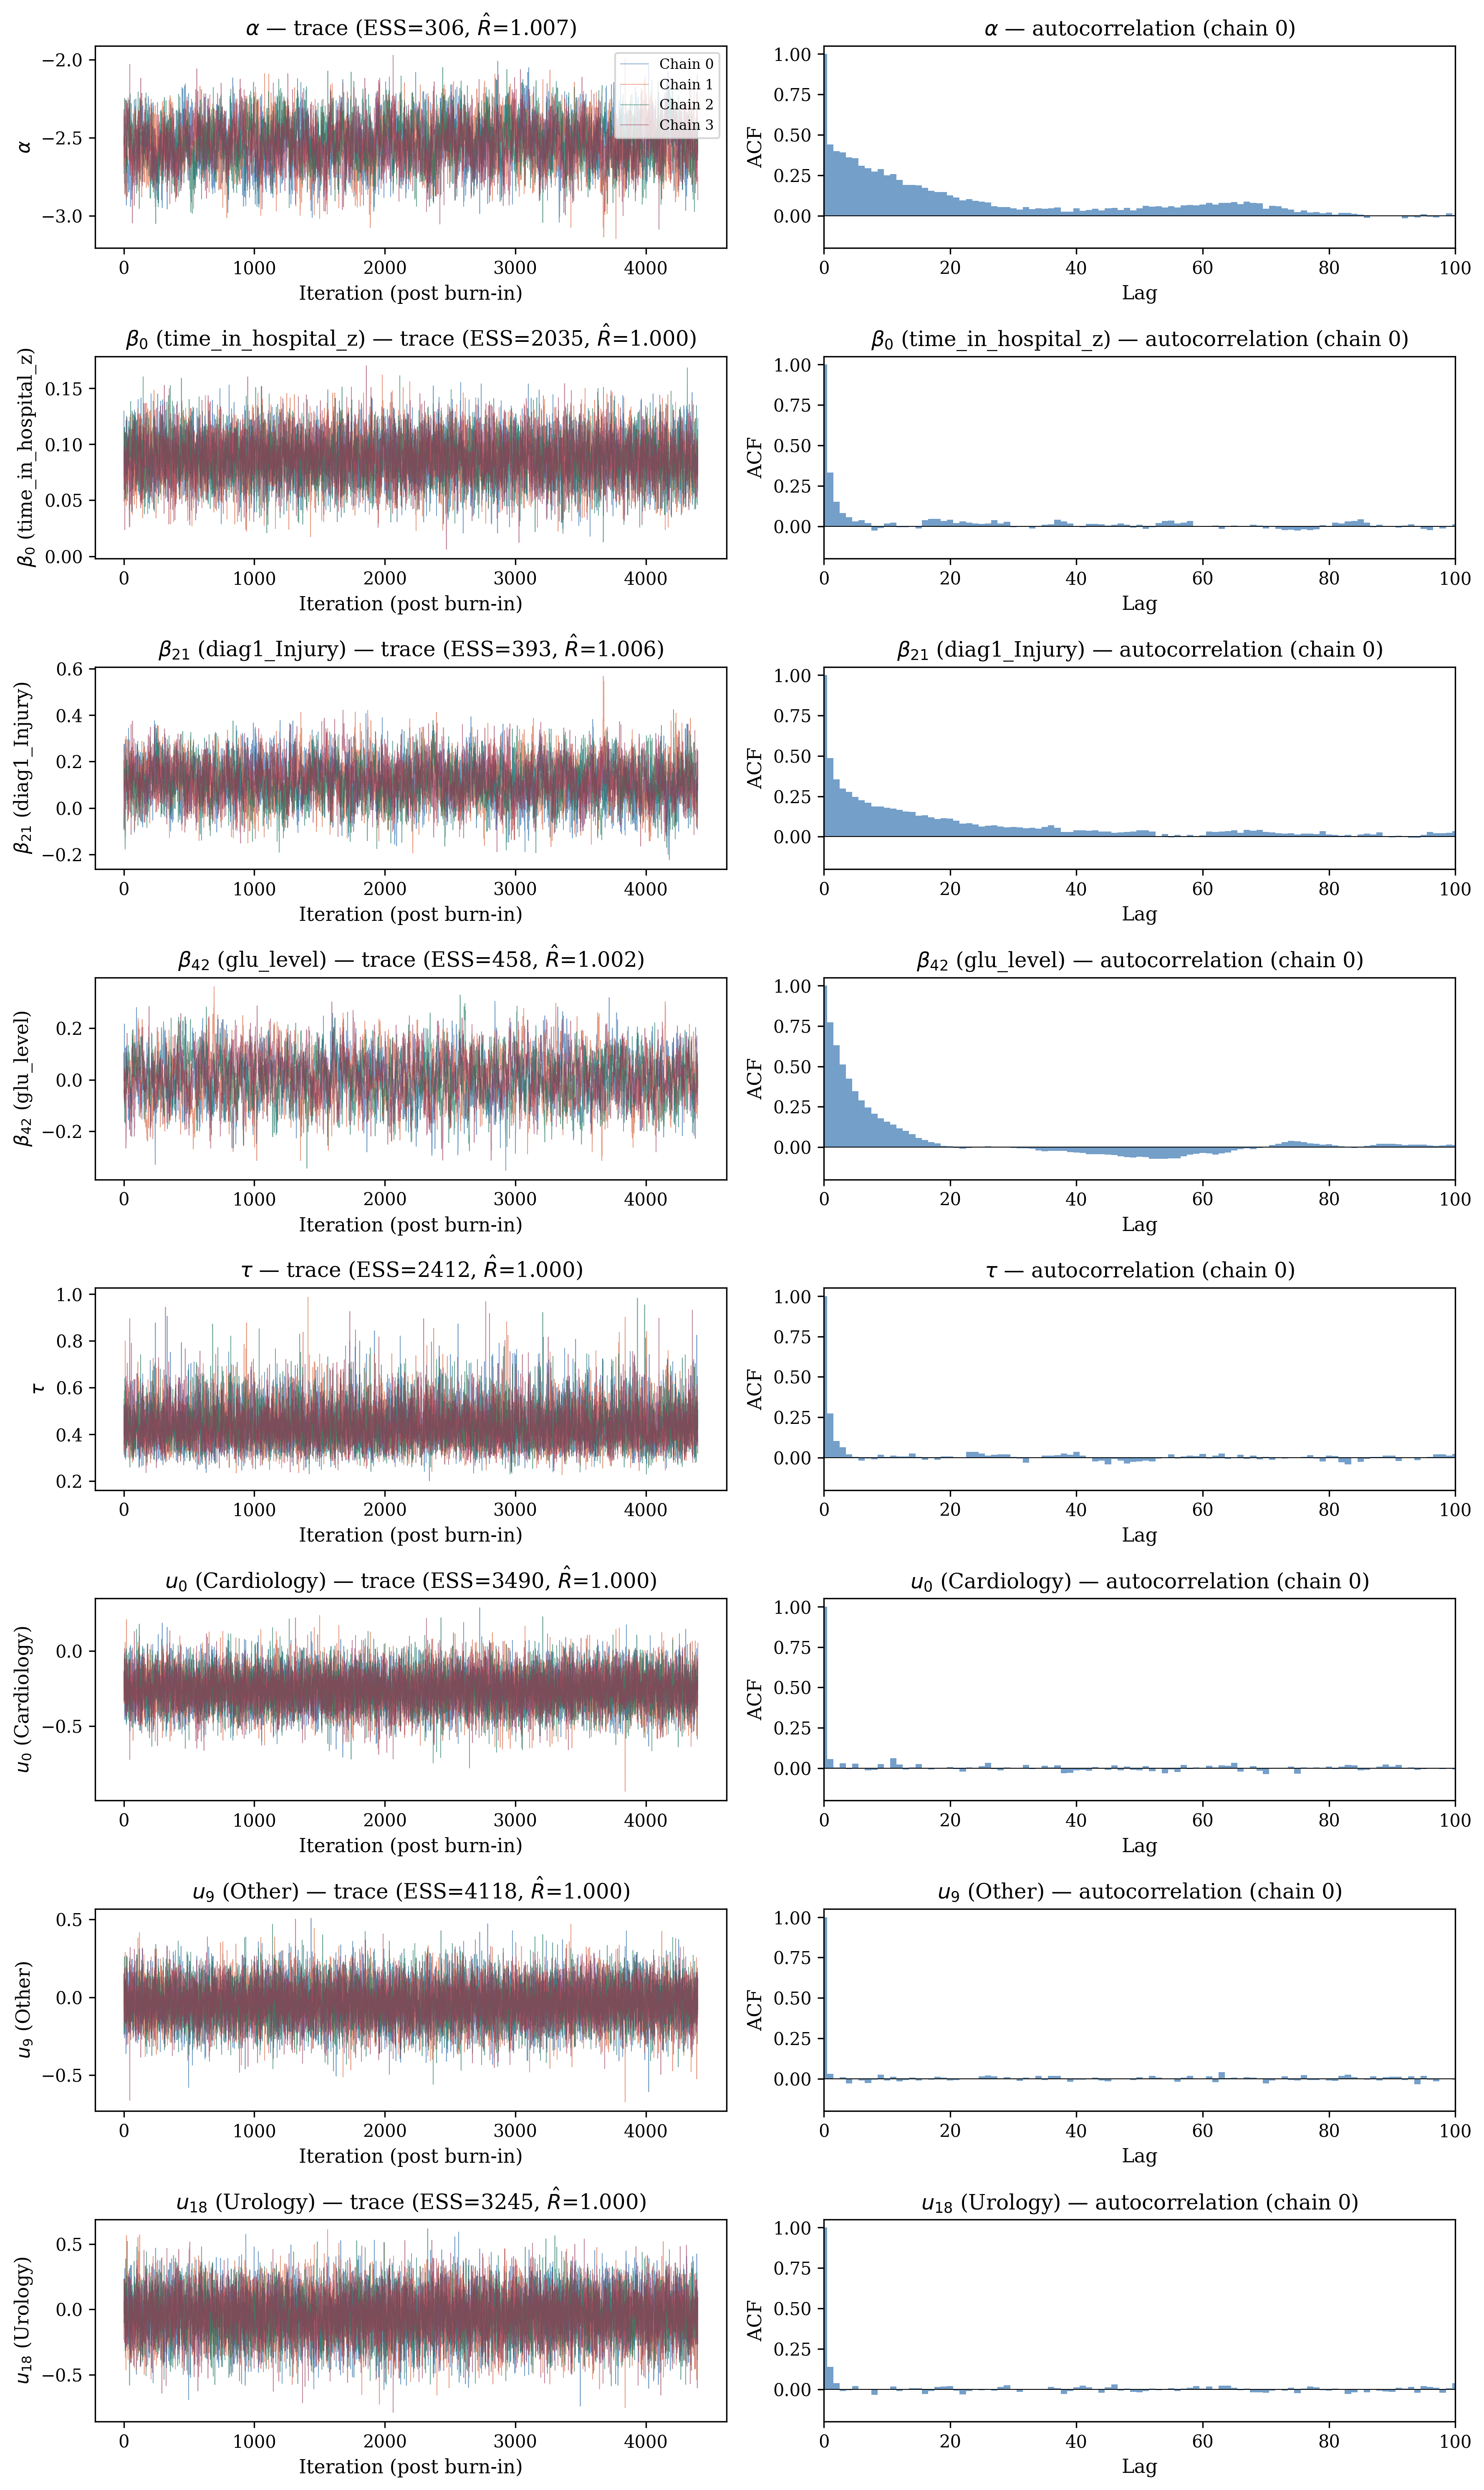
\includegraphics[width=0.88\textwidth,height=0.68\textheight,keepaspectratio]{fig2_trace_plots.png}
\caption{Trace plots (left) and autocorrelation functions (right) for
selected parameters.  The four chains are overlaid in different colours.}
\label{fig:trace}
\end{figure}

\subsection{Effective Sample Size and Cross-Chain Convergence ($\hat{R}$)}

We assess convergence through two complementary quantitative diagnostics:
effective sample size (ESS) and the split-$\hat{R}$ statistic
\citep{gelman1992inference,vehtari2021rank}.

ESS was computed using Geyer's initial monotone sequence estimator, and we
required $\text{ESS} \ge 100$ for every parameter so that posterior means and
quantiles would have acceptable Monte Carlo error. We also monitored
split-$\hat{R}$ and required $\hat{R} < 1.05$ for all parameters, following
standard convergence guidance.

Table~\ref{tab:ess} summarises both diagnostics across parameter types.
All 64 parameters satisfy $\hat{R} < 1.05$, with the maximum
$\hat{R} = 1.013$ (for $\beta_{28}$), well below the
conventional threshold.  All parameters have mean ESS $> 100$;
most exceed 500.  The between-group scale $\tau$ has
ESS $\approx 2{,}412$ and $\hat{R} = 1.000$, indicating
excellent mixing for the key hyperparameter.

\begin{table}[H]
\centering
\caption{Convergence diagnostics by parameter type: effective sample size
(ESS) and split-$\hat{R}$.}
\label{tab:ess}
\begin{tabular}{lrrrr}
\toprule
Parameter block & Min ESS & Median ESS & Max $\hat{R}$ & All $\hat{R} < 1.05$? \\
\midrule
$\alpha$ (intercept) & 245 & 306 & 1.007 & Yes \\
$\bbeta$ (43 fixed effects) & 118 & 866 & 1.013 & Yes \\
$\tau$ (between-group SD) & 2{,}286 & 2{,}412 & 1.000 & Yes \\
$\bu$ (19 random intercepts) & 1{,}593 & 3{,}490 & 1.001 & Yes \\
\bottomrule
\end{tabular}
\end{table}

The lowest ESS values are observed for $\beta_9$ (n\_comorbid\_groups\_z,
ESS $= 251$) and $\beta_{28}$ (comorbid\_circulatory, ESS $= 216$).
These two covariates are mechanically correlated (one counts the number of
comorbidity groups while the other indicates a specific comorbidity), explaining
the higher autocorrelation.  Despite the lower ESS, even 200 effective samples
provide reliable posterior means (Monte Carlo SE $\approx \text{posterior SD} /
\sqrt{200}$, which is small relative to the posterior uncertainty).

The random intercepts $\bu$ have uniformly high ESS (min 1,593), reflecting
the efficiency of the Block~5 joint translation move in breaking the
$\alpha$--$\bu$ correlation.  Without Block~5, preliminary experiments showed
ESS for $\alpha$ dropping below 50, confirming its importance.

% ══════════════════════════════════════════════════════════════════
\section{Results and Inference}
\label{sec:results}
% ══════════════════════════════════════════════════════════════════

\subsection{Fixed Effects}

Table~\ref{tab:fixed} presents the posterior summaries for the most important
fixed effects.  We focus on coefficients whose 95\% credible interval (CrI)
excludes zero.

\begin{table}[H]
\centering
\small
\caption{Key fixed effects: posterior mean, 95\% credible interval, and odds
ratio.  Only coefficients with CrI excluding zero are shown. For standardised
continuous predictors marked ``(z)'', odds ratios correspond to a 1-SD increase.}
\label{tab:fixed}
\begin{tabular}{lrrrr}
\toprule
Variable & Post.\ mean & 95\% CrI & OR & OR 95\% CrI \\
\midrule
Increased risk \\
\quad No.\ prior inpatient (z) & 0.201 & [0.175, 0.227] & 1.22 & [1.19, 1.25] \\
\quad Comorbid neoplasms & 0.415 & [0.198, 0.631] & 1.51 & [1.22, 1.88] \\
\quad A1C measured & 0.352 & [0.154, 0.552] & 1.42 & [1.17, 1.74] \\
\quad Diabetes medication & 0.168 & [0.057, 0.277] & 1.18 & [1.06, 1.32] \\
\quad Age (z) & 0.165 & [0.123, 0.208] & 1.18 & [1.13, 1.23] \\
\quad No.\ diagnoses (z) & 0.154 & [0.111, 0.199] & 1.17 & [1.12, 1.22] \\
\quad Comorbid diabetes & 0.113 & [0.004, 0.224] & 1.12 & [1.00, 1.25] \\
\quad Length of stay (z) & 0.088 & [0.047, 0.128] & 1.09 & [1.05, 1.14] \\
\quad No.\ medications (z) & 0.071 & [0.024, 0.117] & 1.07 & [1.02, 1.12] \\
\midrule
Decreased risk \\
\quad Diag: Neoplasms & $-0.507$ & [$-0.792$, $-0.217$] & 0.60 & [0.45, 0.81] \\
\quad Diag: Respiratory & $-0.360$ & [$-0.519$, $-0.200$] & 0.70 & [0.59, 0.82] \\
\quad Diag: Other & $-0.347$ & [$-0.515$, $-0.181$] & 0.71 & [0.60, 0.83] \\
\quad No.\ procedures (z) & $-0.048$ & [$-0.091$, $-0.006$] & 0.95 & [0.91, 0.99] \\
\bottomrule
\end{tabular}
\end{table}

\paragraph{Interpretation of key risk factors.}
The strongest patient-level predictor of readmission is prior inpatient visits
(OR $= 1.22$ per 1-SD increase), indicating a pattern of recurrent
hospitalisation: a one-standard-deviation increase in prior inpatient visits is
associated with 22\% higher odds of 30-day readmission.

Comorbid neoplasms show the largest effect (OR $= 1.51$), suggesting that
cancer as a secondary diagnosis substantially elevates risk, likely due to
treatment-related complications. In contrast, primary neoplasm diagnoses are
protective (OR $= 0.60$), potentially reflecting structured oncology follow-up
and closer post-discharge care. This contrast underscores the importance of
distinguishing primary versus secondary diagnoses. Age (OR $= 1.18$ per 1-SD
increase), number of diagnoses (OR $= 1.17$ per 1-SD increase), and length of
stay (OR $= 1.09$ per 1-SD increase) capture overall medical complexity, with
older and more multimorbid patients at higher risk. The A1C measurement
indicator (OR $= 1.42$) likely reflects confounding by indication: patients
with more severe or poorly controlled diabetes are both more likely to be
tested and more likely to be readmitted. Similarly, diabetes medication use
(OR $= 1.18$) appears to proxy disease severity rather than a causal effect.

Non-significant predictors include sex, race, and insulin use. The null effect for race suggests that observed disparities in unadjusted analyses are largely explained by differences in clinical characteristics rather than race itself. Insulin use is also not independently associated with readmission after accounting for overall treatment intensity and disease severity.

\subsection{Specialty-Level Heterogeneity}

\paragraph{Between-group scale $\tau$.}
The posterior mean of $\tau$ is 0.437 (SD $= 0.090$, 95\% CrI [0.298, 0.644]),
with $P(\tau > 0.1 \mid \by) = 1.0$ and $P(\tau > 0.2 \mid \by) = 1.0$.
This provides strong evidence that specialty-level heterogeneity persists after
adjusting for patient covariates.  The posterior density of $\tau$ is clearly
concentrated away from zero, ruling out the complete-pooling model ($\tau = 0$).
The moderate right skew reflects the prior's constraint to positive values and
the limited number of groups ($J = 19$).

\begin{figure}[H]
\centering
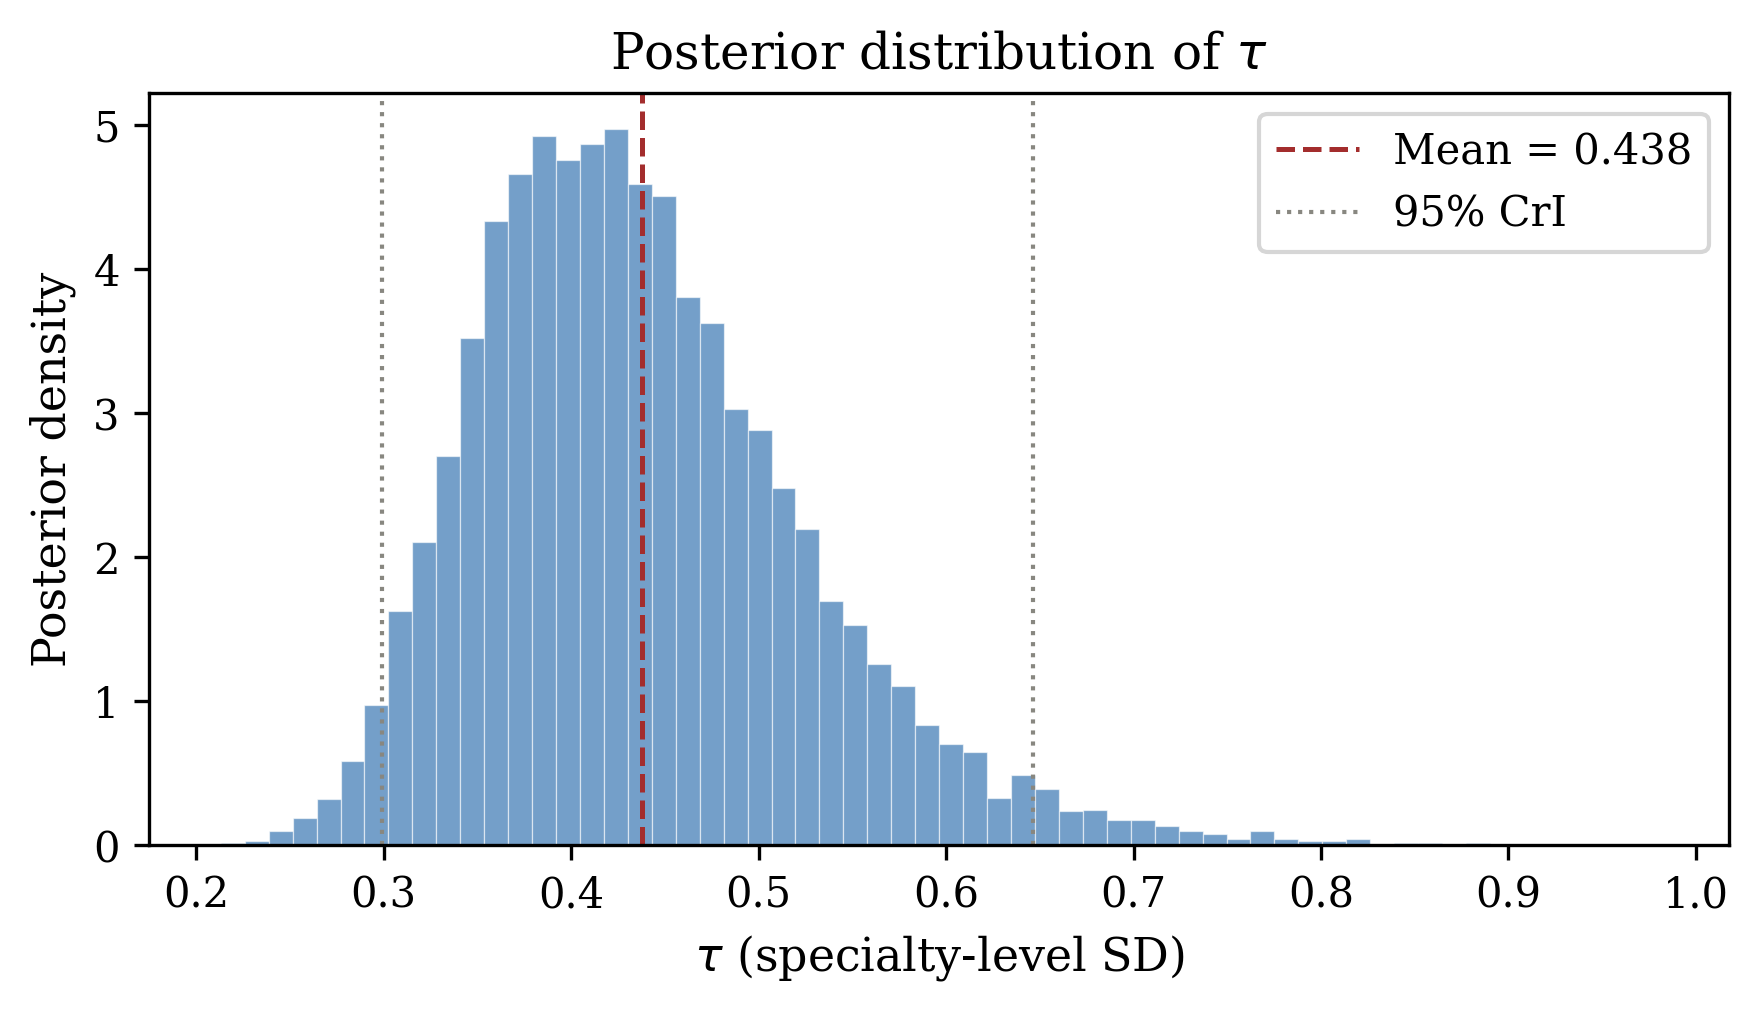
\includegraphics[width=0.55\textwidth]{fig_tau_posterior.png}
\caption{Posterior density of the between-specialty standard deviation
$\tau$.  The distribution is concentrated well above zero, providing strong
evidence for specialty-level heterogeneity.}
\label{fig:tau-posterior}
\end{figure}

\paragraph{Specialty random effects.}

Physical Medicine and Rehabilitation (PMR) shows a markedly elevated random
intercept ($\hat{u} = 1.32$, 95\% CrI $[0.99, 1.67]$) and is the only specialty
with an interval entirely above zero. PMR also has the highest raw
readmission rate (32.3\%), and its adjusted random intercept remains strongly
positive after accounting for patient covariates. This likely reflects its
patient population with high medical complexity and vulnerability to
post-discharge complications. In contrast, Surgery-Cardiovascular/Thoracic
exhibits a significantly negative effect ($\hat{u} = -0.58$, 95\% CrI
$[-0.99, -0.21]$), potentially due to structured post-operative care and
follow-up protocols. Psychiatry shows a modest positive effect ($\hat{u} =
0.22$) with a credible interval overlapping zero, indicating no clear
deviation from the average after adjustment. Similarly, Emergency/Trauma and
Internal Medicine have effects close to zero ($\hat{u} \approx 0.03$ and
$\hat{u} \approx -0.03$), as expected for large groups with stable estimates.
Most other specialties have intervals that include zero, suggesting their
readmission risks are broadly consistent with the overall average and that the
model primarily identifies truly extreme groups rather than spurious
differences.

\begin{figure}[H]
\centering
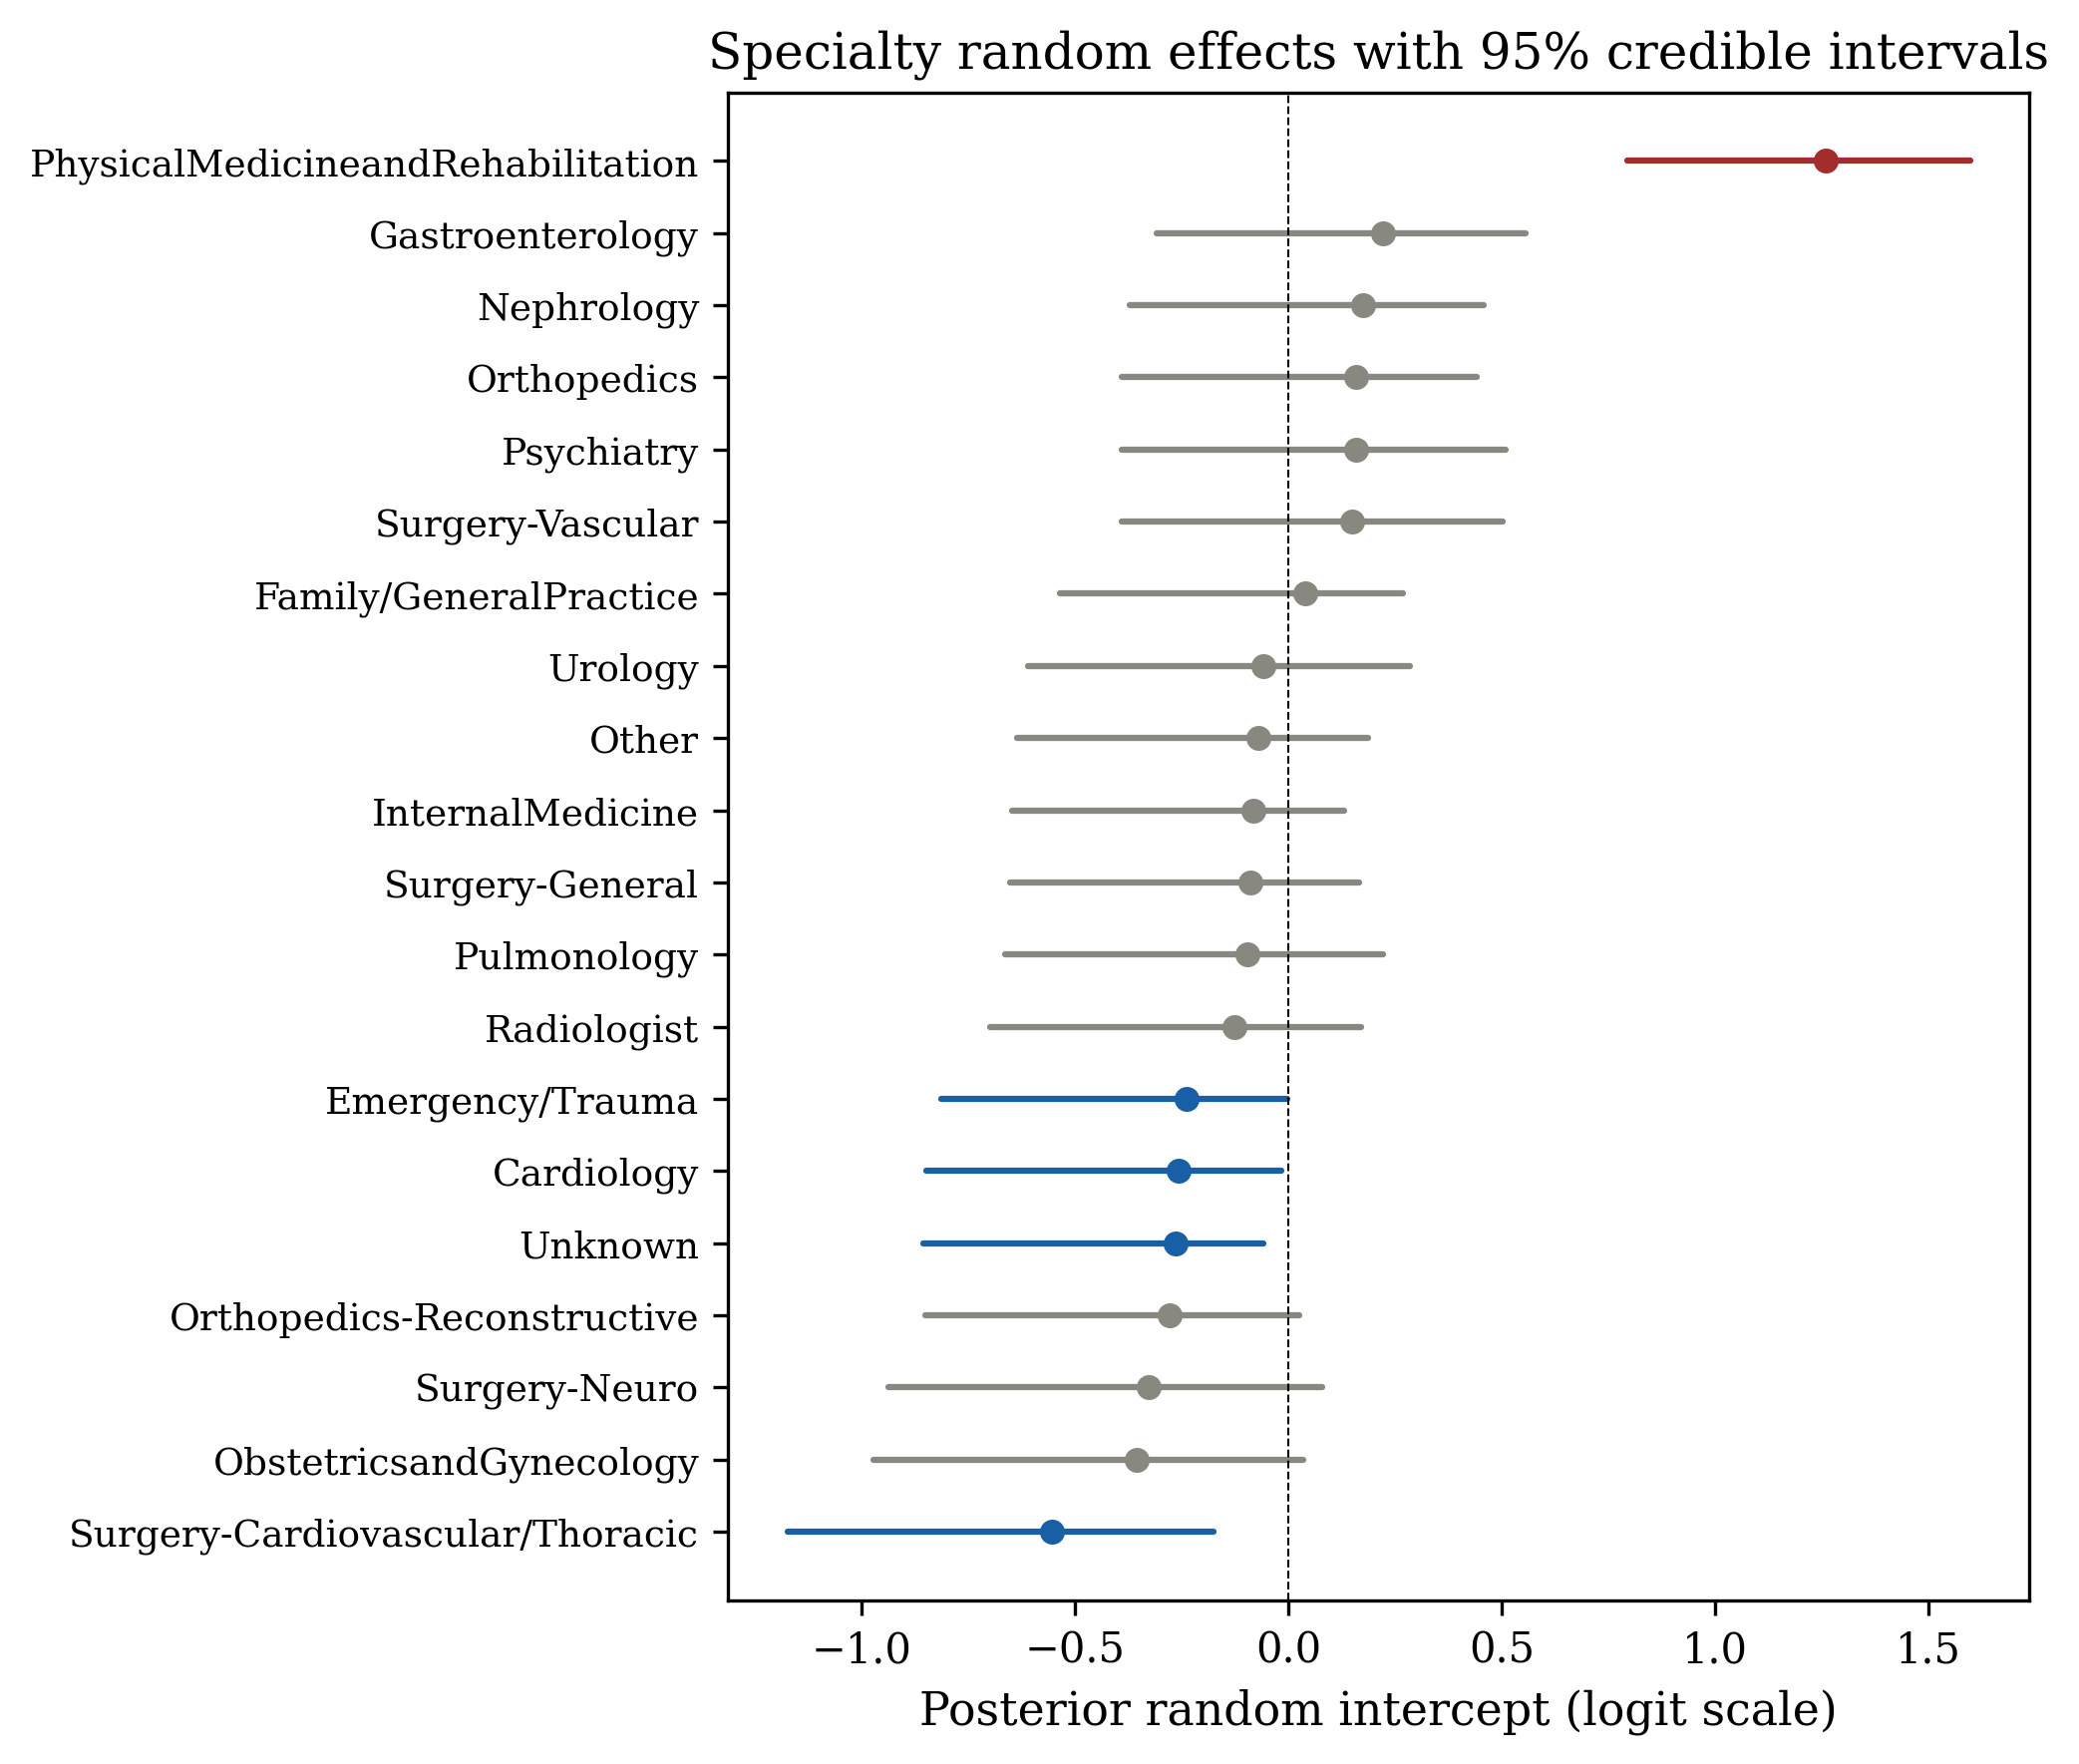
\includegraphics[width=0.75\textwidth]{fig4_specialty_random_effects.png}
\caption{Specialty random effects (posterior mean and 95\% CrI).  Red:
interval entirely above zero; blue: entirely below zero; grey: includes zero.}
\label{fig:forest}
\end{figure}

\subsection{Model Comparison}

Table~\ref{tab:comparison} compares three models on in-sample predictive
performance.

\begin{table}[H]
\centering
\caption{Model comparison metrics.}
\label{tab:comparison}
\begin{tabular}{lcccc}
\toprule
Model & AUC & Brier Score & Log-Loss & Calibration Slope \\
\midrule
No specialty (baseline) & 0.629 & 0.0852 & 0.307 & 1.003 \\
Specialty fixed effects & 0.641 & 0.0846 & 0.305 & 0.997 \\
Bayesian hierarchical & 0.641 & 0.0846 & 0.305 & 1.024 \\
\bottomrule
\end{tabular}
\end{table}

The hierarchical model matches fixed-effects performance on in-sample
discrimination (AUC $= 0.641$) and in-sample calibration (Brier $= 0.0846$),
while offering the advantages of partial pooling for small groups and a
coherent estimate of between-group variability. The fact that both the
specialty fixed-effects model and the hierarchical model improve over the
baseline in these in-sample metrics (AUC $0.641$ vs.\ $0.629$) suggests that
specialty-level information adds predictive signal beyond patient-level
covariates alone. Because these summaries are evaluated in-sample, they should
be interpreted as evidence of improved model fit rather than out-of-sample
superiority. The calibration slope of 1.024 for the hierarchical model
indicates slight in-sample under-confidence (predicted probabilities are
marginally too conservative), but is close to the ideal value of 1.0.

\paragraph{DIC.}  The Deviance Information Criterion \citep{spiegelhalter2002dic}
provides a Bayesian measure of model fit penalised by complexity.
Define the deviance
$D(\btheta) = -2\sum_{i=1}^{N}\bigl[y_i\eta_i - \log(1+e^{\eta_i})\bigr]$,
where $\btheta = (\alpha,\bbeta,\bu)$. Then:
\begin{align}
  \bar{D} &= \mathbb{E}_{\btheta\mid\by}\bigl[D(\btheta)\bigr]
    \approx \frac{1}{S}\sum_{s=1}^{S}D(\btheta^{(s)}), \\
  p_D &= \bar{D} - D(\bar{\btheta}), \qquad
  \text{DIC} = \bar{D} + p_D,
\end{align}
where $\bar{\btheta} = \mathbb{E}[\btheta\mid\by]$ and $p_D$ is the
\textbf{effective number of parameters}.

For the hierarchical model,
$\text{DIC} = 23{,}254$ with $p_D = 60.5$.  The nominal parameter count is 64
($1 + 43 + 19 + 1$); $p_D < 64$ confirms that the hierarchical
prior induces shrinkage on the random intercepts, as expected.  The
difference $64 - 60.5 = 3.5$ represents the effective reduction in model
complexity due to partial pooling: approximately 3--4 of the 19 random
intercepts are substantially shrunk toward zero, reducing their effective
contribution to model complexity.  This is consistent with the observation
that most specialties have credible intervals overlapping zero---these
``near-zero'' intercepts contribute less than one effective parameter each.

\subsection{Posterior Predictive Checks}

We assess model adequacy by simulating replicated datasets from the
posterior predictive distribution. For each of $S_{\text{rep}} = 200$
posterior draws $\btheta^{(s)} = (\alpha^{(s)}, \bbeta^{(s)}, \bu^{(s)})$, we
compute fitted probabilities, simulate a replicated dataset, and evaluate two
test statistics: the overall readmission rate $T_1 = \bar{y}^{\text{rep}}$
and the standard deviation of specialty-specific rates
$T_2 = \text{SD}$ of group-level rates.
The Bayesian $p$-value is
$p_B = \Pr\bigl(T(\by^{\text{rep}}) \ge T(\by^{\text{obs}})\bigr)$;
values near 0.5 indicate good calibration, while values near 0 or 1 indicate
systematic model misfit.

The observed overall readmission rate (9.60\%) falls squarely within the
replicated distribution (Bayesian $p$-value $= 0.500$), indicating that the
model reproduces the marginal readmission rate without systematic over- or
under-prediction.  A $p$-value of exactly 0.500 is ideal---it means the
observed statistic is at the median of the posterior predictive distribution.

The observed specialty-rate variability (standard deviation of group-level
rates) is also well-captured ($p$-value $= 0.245$), confirming that the
hierarchical structure with estimated $\tau$ adequately represents the degree
of between-specialty variation in the data.  A $p$-value of 0.245 indicates
that the model generates slightly more specialty-level variability than
observed in 24.5\% of replications---well within the acceptable range.  If the
model had underestimated $\tau$, this $p$-value would be close to 0;
overestimation would push it toward 1.

Both checks confirm adequate model fit and provide no evidence of systematic
misspecification.

\begin{figure}[H]
\centering
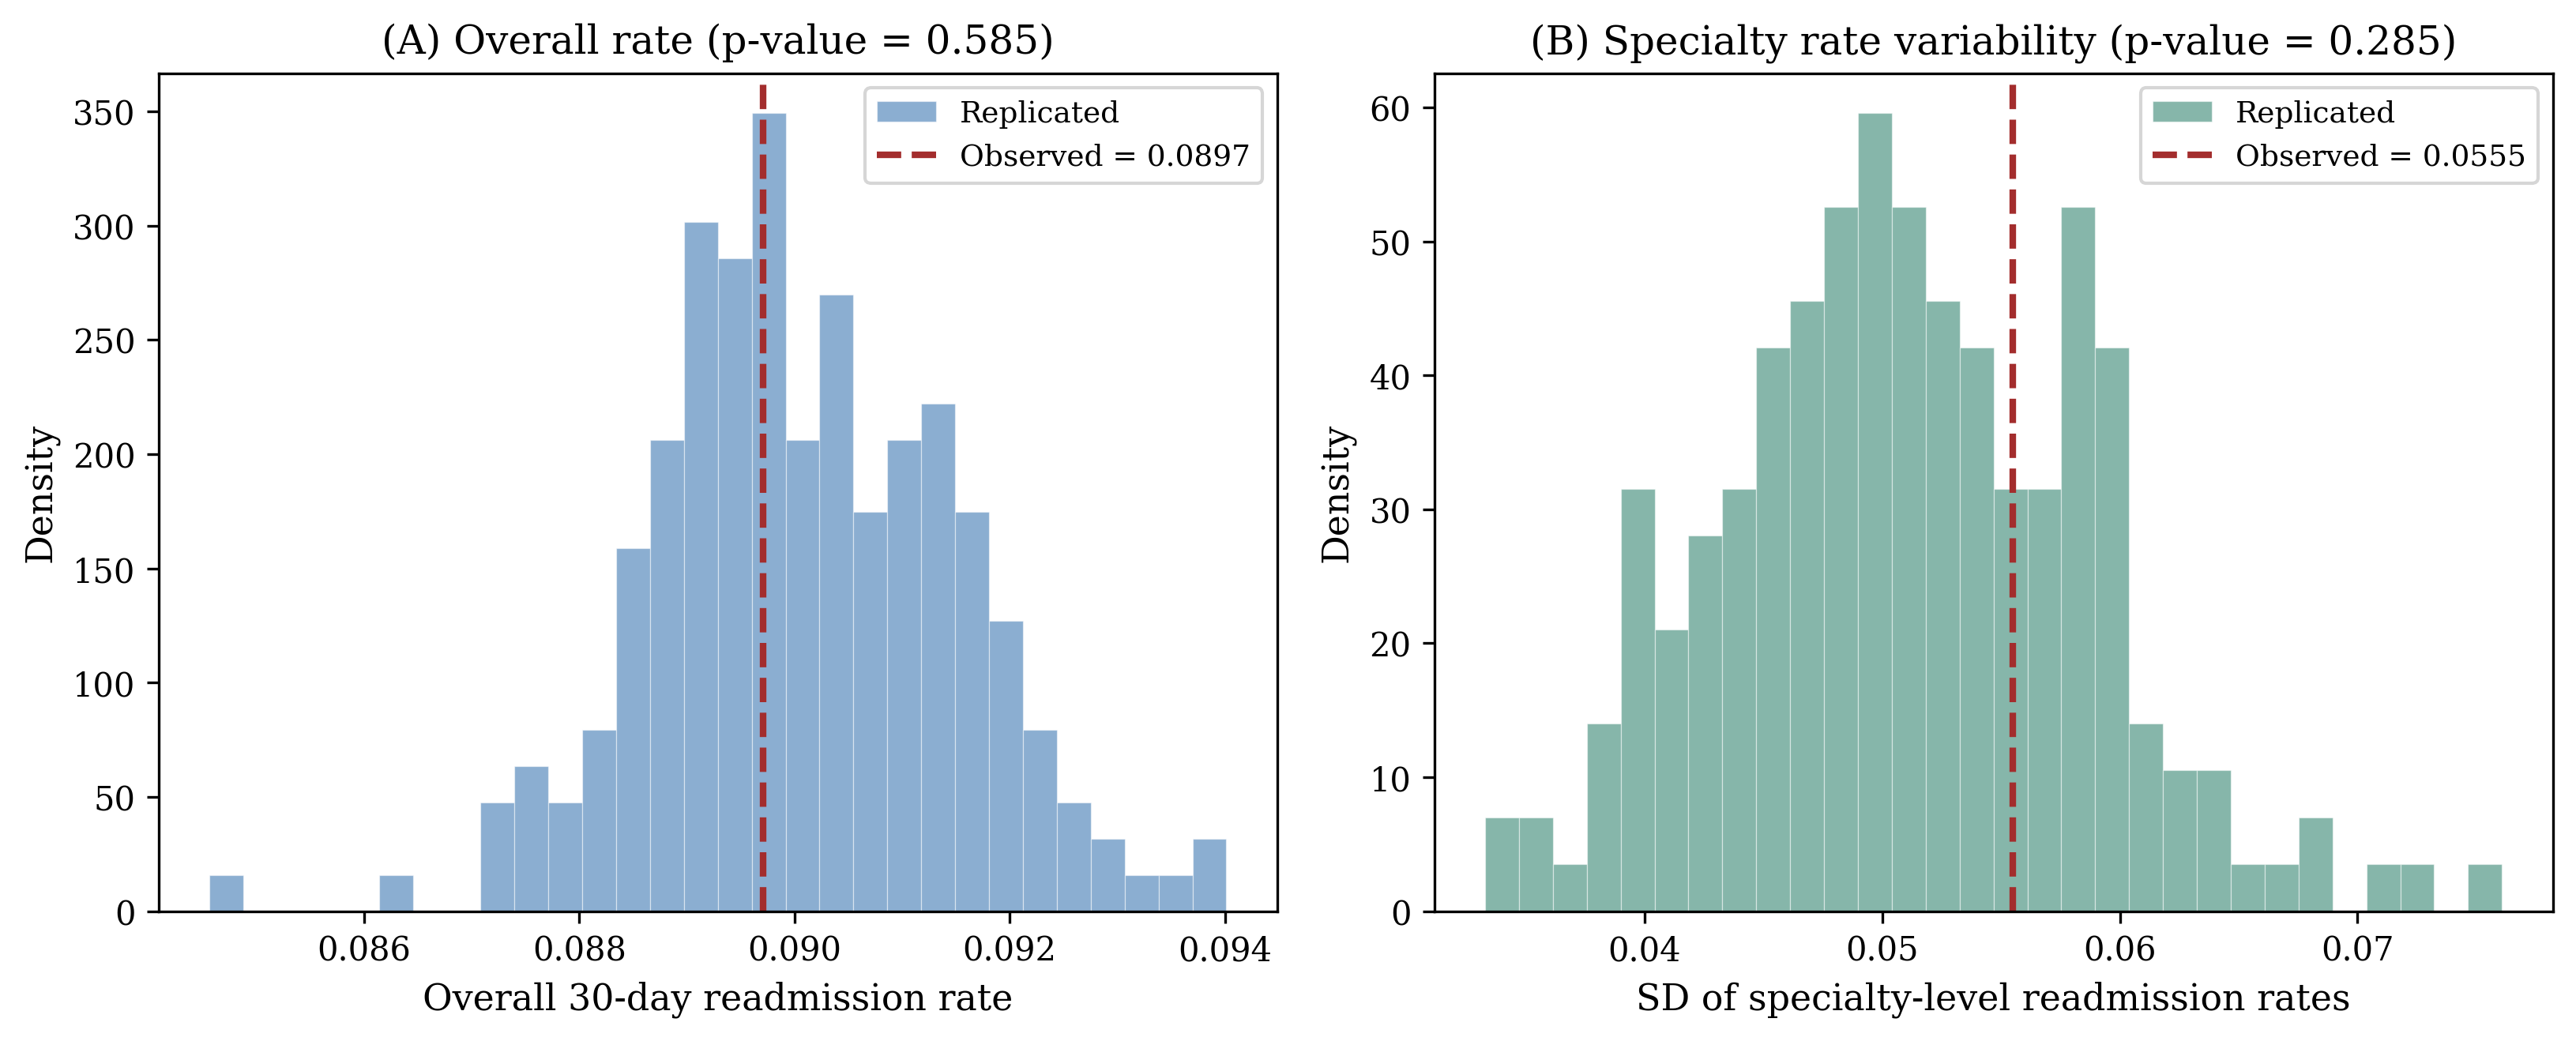
\includegraphics[width=0.92\textwidth]{fig5_posterior_predictive.png}
\caption{Posterior predictive checks.  (A) Overall readmission rate.
(B) Standard deviation of specialty-level rates.  Dashed red lines show
observed values.}
\label{fig:ppc}
\end{figure}

% ══════════════════════════════════════════════════════════════════
\section{Sensitivity Analysis}
\label{sec:sensitivity}
% ══════════════════════════════════════════════════════════════════

We assess robustness to prior specification by re-running the sampler under
three alternative configurations, summarised in Table~\ref{tab:sensitivity}.

\begin{table}[H]
\centering
\small
\caption{Prior sensitivity configurations.}
\label{tab:sensitivity}
\begin{tabular}{llll}
\toprule
Label & Change & $s_\beta$ & $\tau$ prior \\
\midrule
Baseline & --- & 2.5 & $\HalfNormal(0, 1.0)$ \\
A1 & Wider $\beta$ prior & 5.0 & $\HalfNormal(0, 1.0)$ \\
B1 & Wider $\tau$ prior & 2.5 & $\HalfNormal(0, 2.5)$ \\
B2 & Heavy-tailed $\tau$ prior & 2.5 & $\HalfCauchy(0, 2.5)$ \\
\bottomrule
\end{tabular}
\end{table}

The posterior of $\tau$ is virtually identical across all four configurations
(posterior means: 0.437, 0.437, 0.441, 0.440; posterior SDs: 0.090, 0.090,
0.092, 0.091).  The 95\% credible intervals overlap almost perfectly across
configurations, confirming that the data overwhelm the prior for this
hyperparameter.  Even the heavy-tailed Half-Cauchy prior (B2), which places
substantially more mass on large values of $\tau$, produces a posterior that
is indistinguishable from the baseline---strong evidence that the posterior
of $\tau$ is likelihood-dominated with $J = 19$ groups.

Key fixed effects are numerically unchanged across all configurations. For
\texttt{comorbid\_neoplasms}, \texttt{A1C\_measured}, and
\texttt{number\_inpatient\_z}, the posterior means vary by less than 0.001
across the four prior settings, confirming that with $N = 37{,}964$
observations the likelihood dominates the prior on $\bbeta$. Likewise, the PMR
random intercept remains the only clearly elevated specialty effect, with
posterior means ranging from 1.31 to 1.33, well within Monte Carlo error.

\begin{figure}[H]
\centering
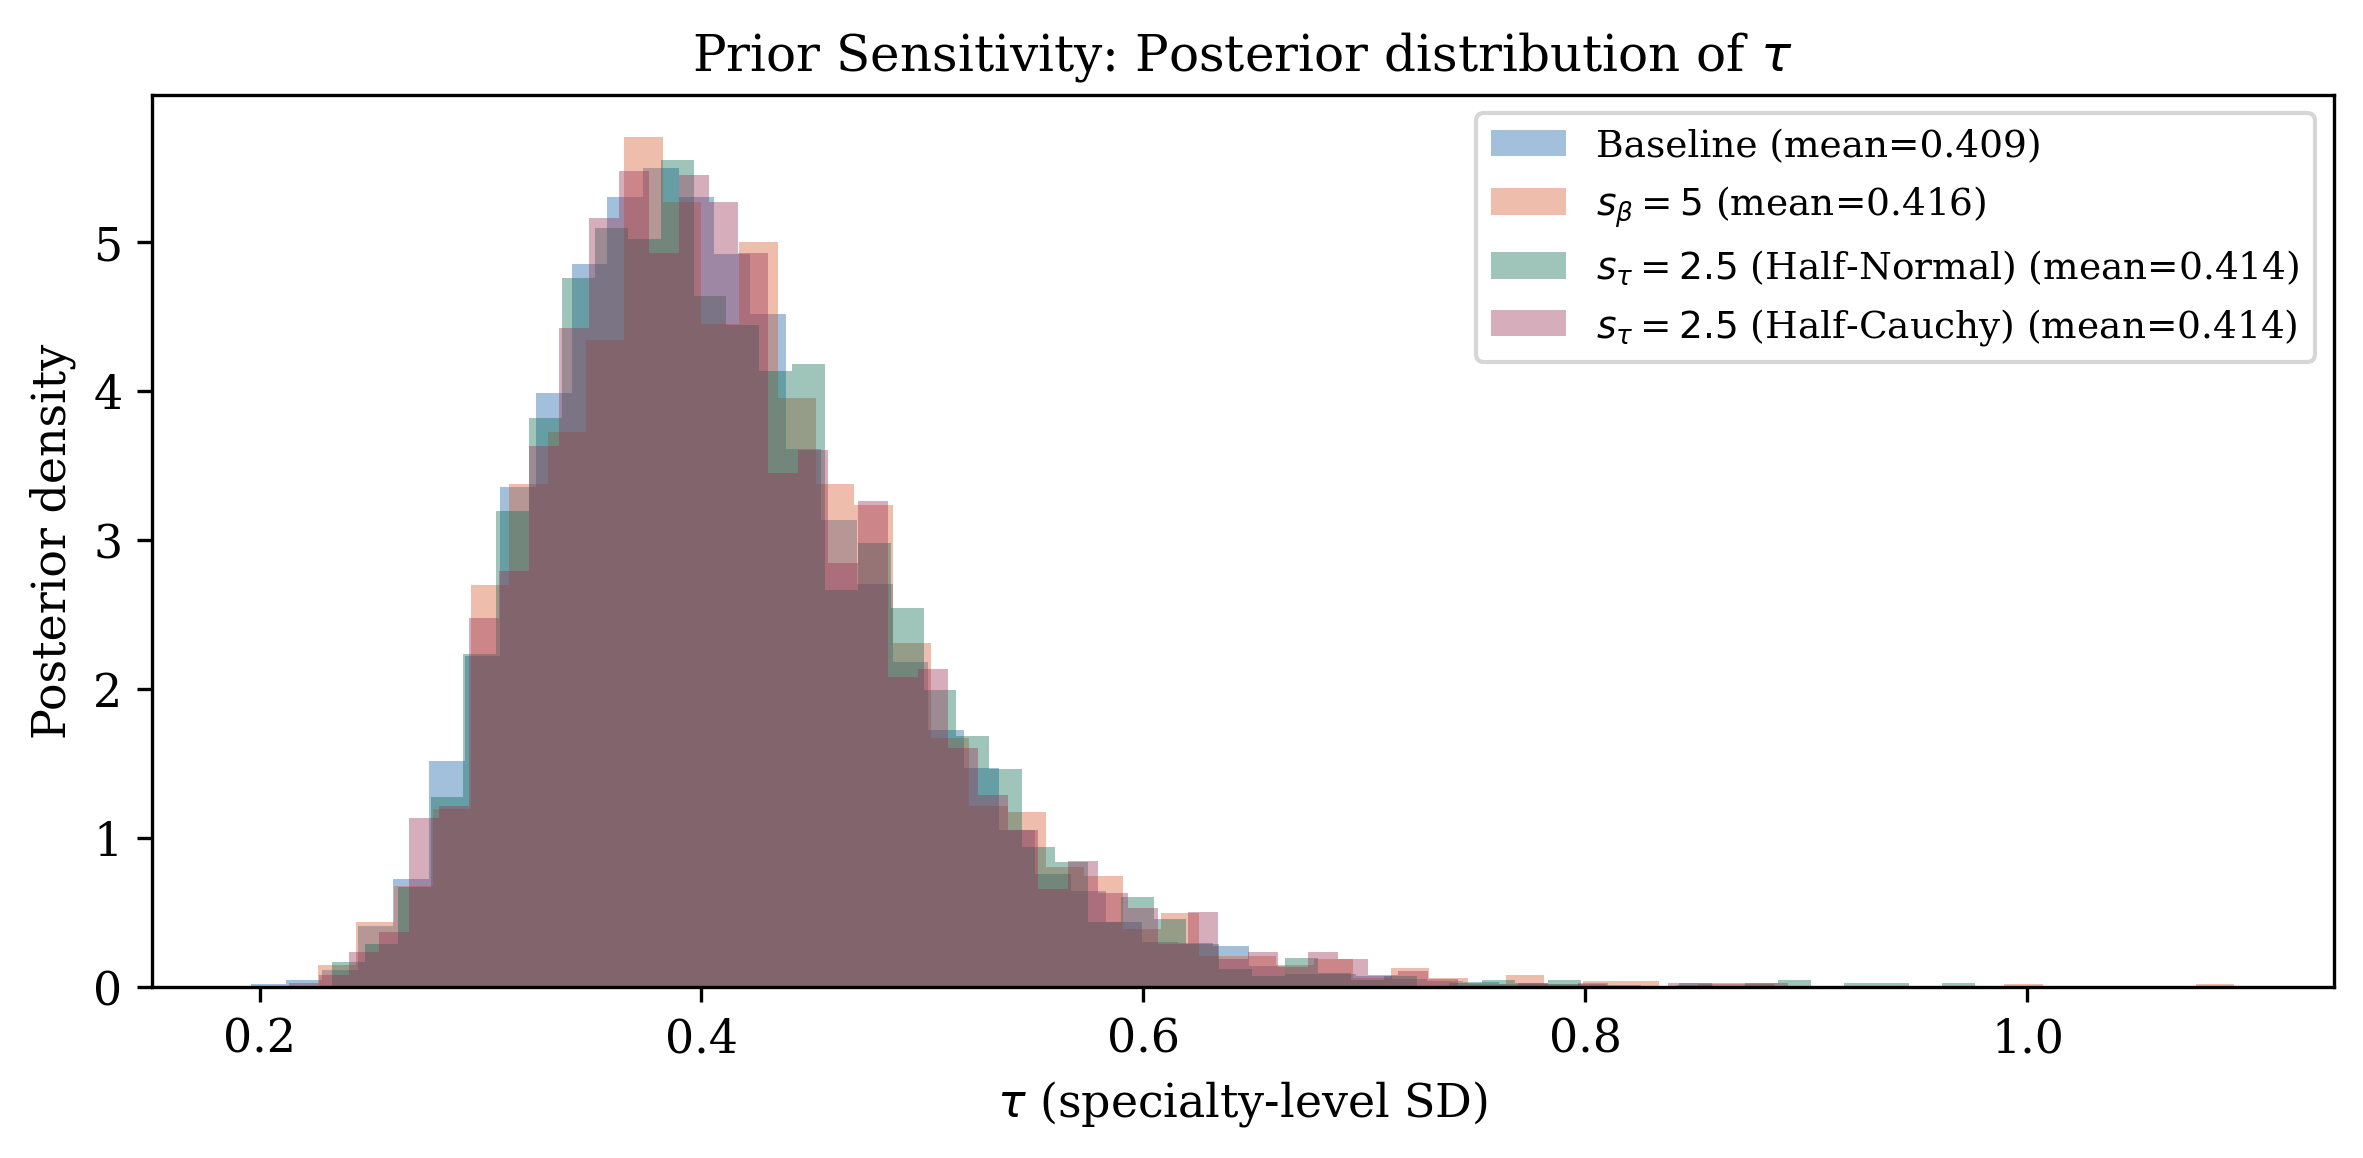
\includegraphics[width=0.78\textwidth]{fig6_sensitivity_tau.png}
\caption{Posterior distribution of $\tau$ under four prior configurations.}
\label{fig:sens-tau}
\end{figure}

\begin{figure}[H]
\centering
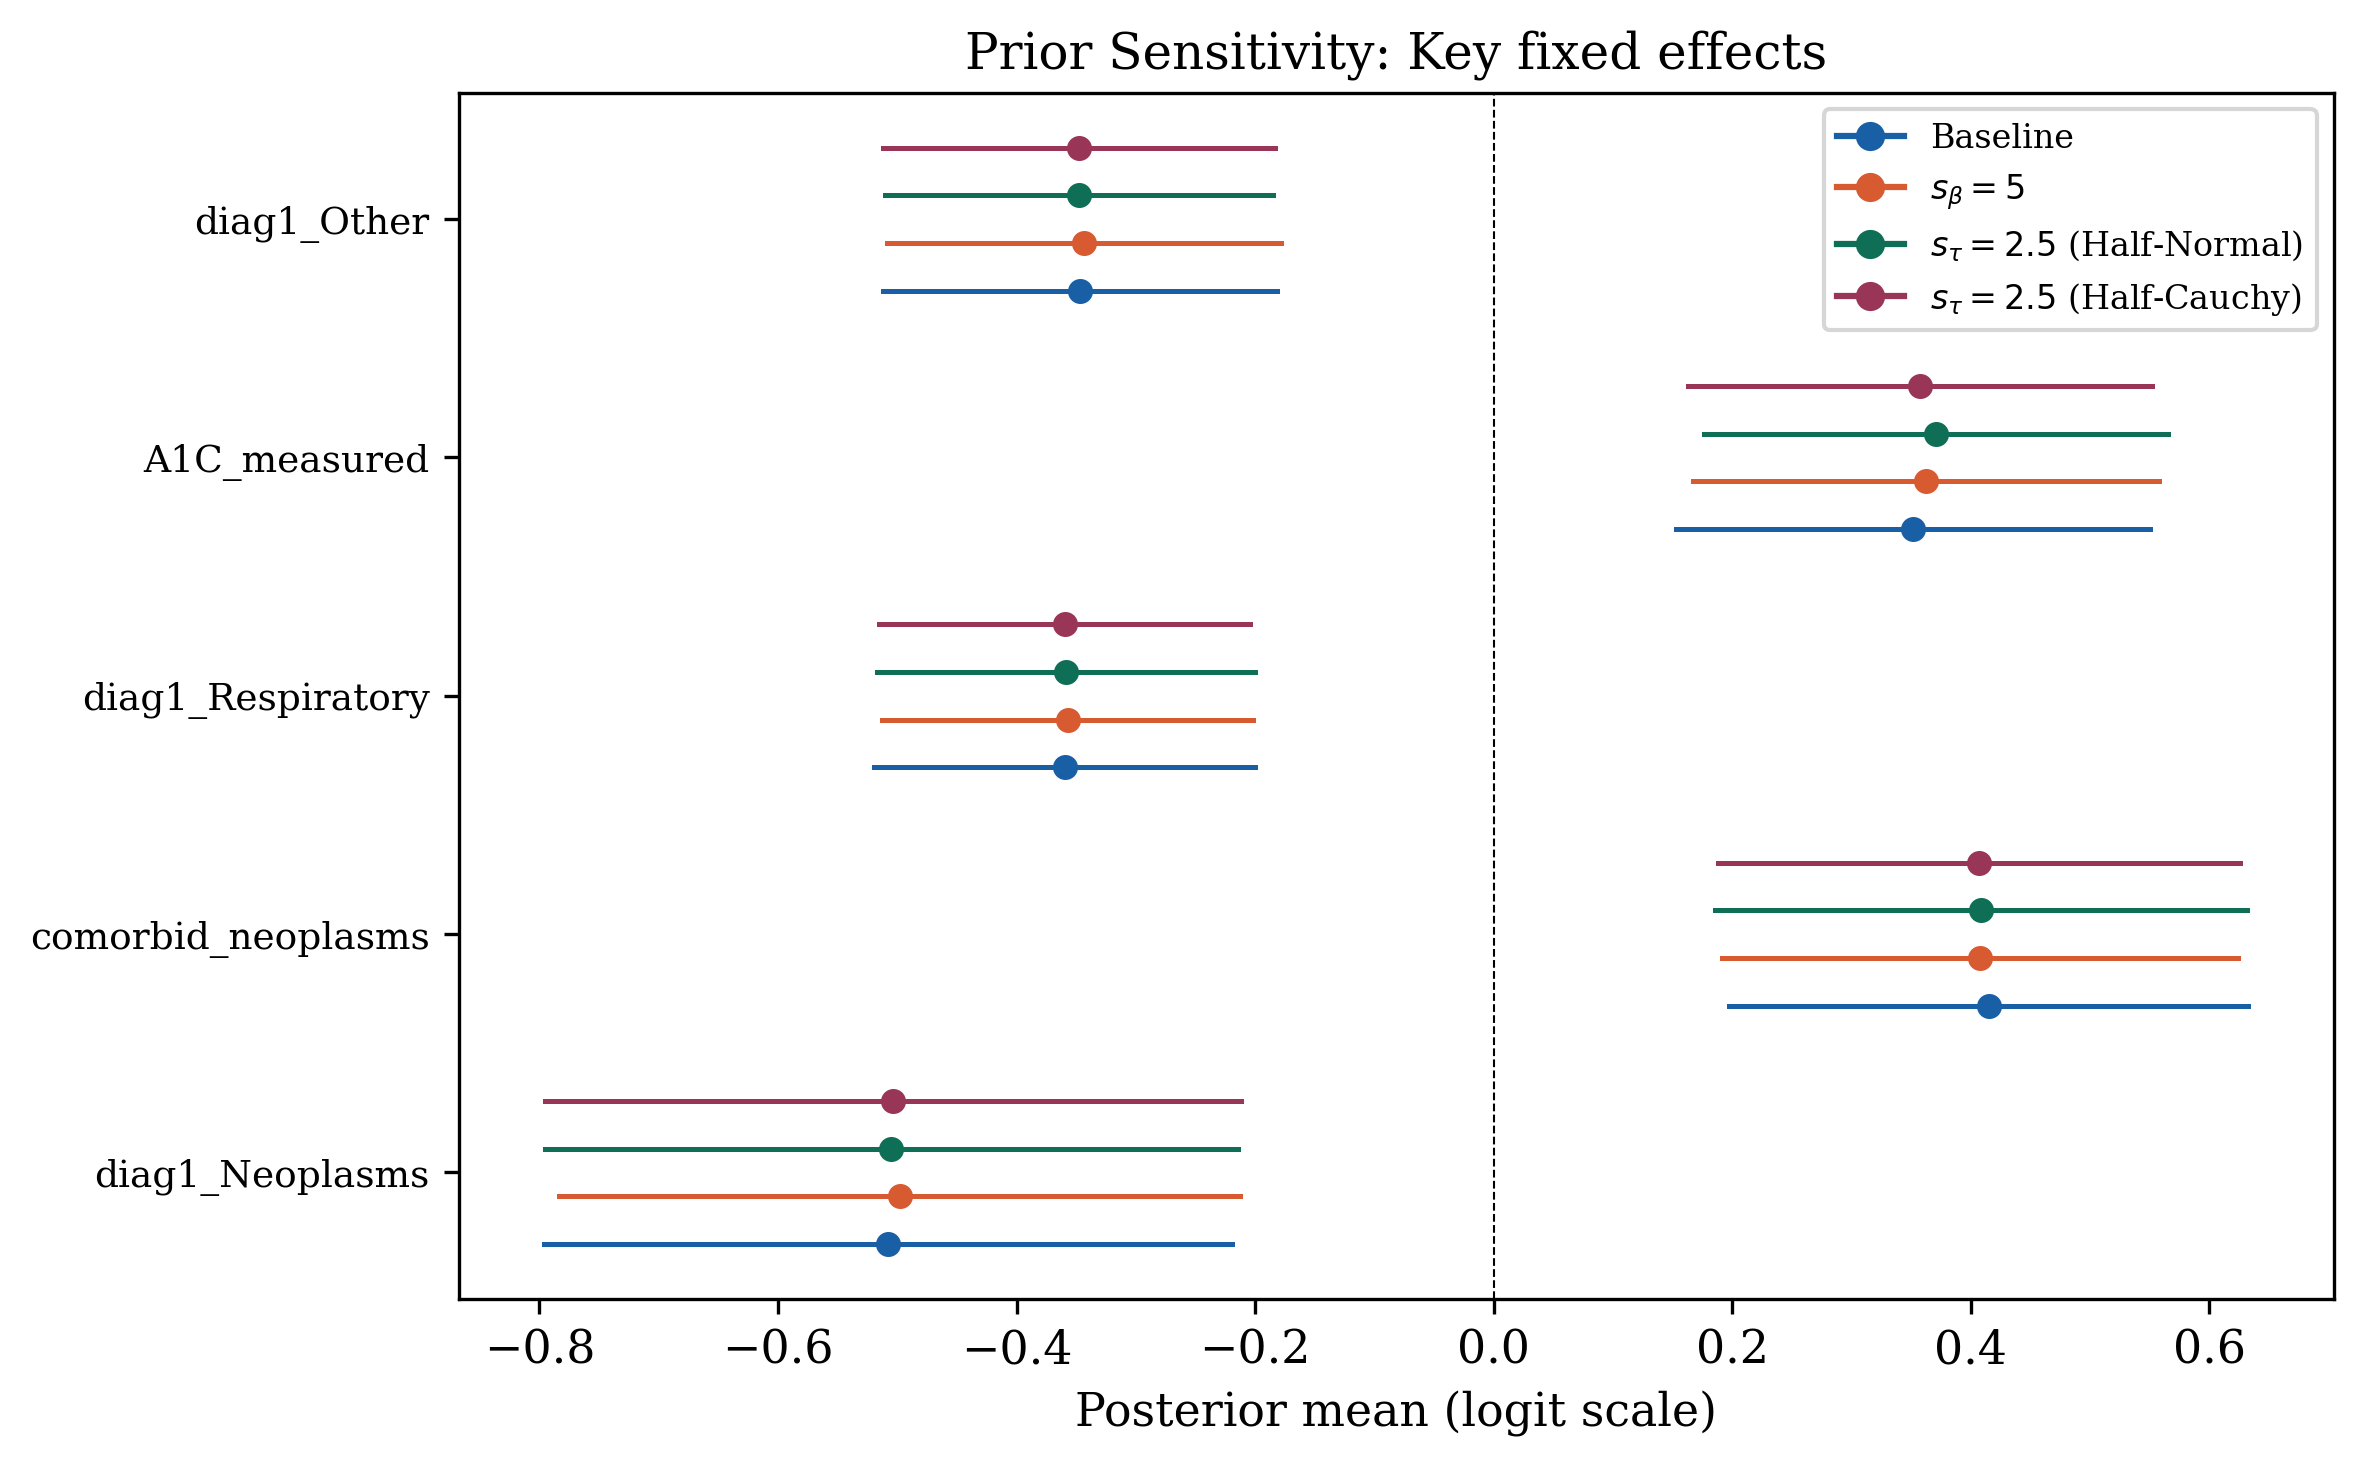
\includegraphics[width=0.78\textwidth]{fig7_sensitivity_beta.png}
\caption{Posterior means and 95\% CrI for key fixed effects under four prior
configurations.}
\label{fig:sens-beta}
\end{figure}

All substantive findings---the magnitude of $\tau$, the significance of key
fixed effects, and the identification of PMR as an outlier---are robust to
reasonable variation in prior specification.  This is consistent with the
large sample size ($N = 37{,}964$) providing strong likelihood information
that dominates the weakly informative priors.  The sensitivity analysis
validates the choice of priors in Section~\ref{sec:model}: conclusions
would be identical under substantially different prior beliefs.

% ══════════════════════════════════════════════════════════════════
\section{Discussion}
\label{sec:discussion}
% ══════════════════════════════════════════════════════════════════

\subsection{Summary}

Our analysis yields three main findings. Medical specialty contributes meaningfully to readmission risk beyond patient characteristics, with between-specialty variability $\tau = 0.437$ (95\% CrI [0.298, 0.644]) and $P(\tau > 0.2 \mid y) = 1.0$, indicating that negligible specialty effects are strongly unsupported by the data. Physical Medicine and Rehabilitation (PMR) emerges as a clear outlier, with substantially elevated risk ($u = 1.32$) and a raw readmission rate of 32.3\%, even after adjustment, likely reflecting a highly complex patient population and highlighting a potential target for intervention. At the patient level, prior inpatient visits, comorbid neoplasms, A1C measurement, age, and number of diagnoses are the strongest predictors, collectively pointing to medical complexity as the primary driver of readmission risk.

\subsection{Clinical Implications}

The identification of specialty-level heterogeneity has direct implications for quality improvement. Rather than applying uniform readmission reduction strategies, hospitals could implement targeted post-discharge protocols for high-risk groups such as PMR patients, including enhanced transitional care and closer outpatient follow-up. Practices from specialties with lower readmission risk, such as cardiovascular surgery, could be examined as potential models for broader adoption. In addition, posterior predictive probabilities from the hierarchical model could be used to identify high-risk patients at discharge and guide proactive intervention.

The contrasting effects of neoplasms further highlight the importance of clinical context. Comorbid neoplasms as a secondary diagnosis substantially increase readmission risk, whereas neoplasms as a primary diagnosis appear protective, suggesting that multimorbidity management, particularly at the intersection of cancer and diabetes, requires focused clinical attention.


\subsection{Partial Pooling and Likelihood- vs.\ Prior-Driven Behavior}

Different parameter blocks exhibit different degrees of prior influence,
reflecting the hierarchical model's structure. With $N = 37{,}964$
observations and weakly informative priors ($s_\beta = 2.5$), the fixed
effects $\bbeta$ are overwhelmingly likelihood-driven: the prior precision
$1/s_\beta^2 = 0.16$ is negligible relative to the information in the data,
and widening the prior to $s_\beta = 5$ leaves posterior summaries virtually
unchanged. By contrast, the random intercepts $u_j$ are only partially pooled,
as described by Equation~\eqref{eq:shrinkage}: large groups such as Internal
Medicine ($n = 10{,}975$) have shrinkage weights close to one, whereas smaller
groups such as PMR ($n = 288$) are pulled more noticeably toward zero. Even
after this shrinkage, PMR remains strongly elevated, showing that the signal is
substantial rather than an artefact of small-sample noise. The between-group
scale $\tau$ is learned from the empirical dispersion of the $u_j$'s, and the
sensitivity analysis shows that its posterior changes little when the
hyperprior is widened or replaced by a Half-Cauchy. Together, these patterns
illustrate the main advantage of the hierarchical model: it borrows strength
for small specialties without washing out genuine between-specialty
heterogeneity.

\subsection{Limitations}

Several limitations should be noted. The exclusion of 45.7\% of encounters with missing specialty may introduce selection bias if these patients differ systematically from those with observed specialty. The model assumes constant covariate effects across specialties, although effects such as comorbidity burden may vary in practice. Temporal and hospital-level variation are not explicitly modelled despite the data spanning 10 years across 130 hospitals, so estimated specialty effects may partly reflect unmeasured factors. As an observational study, specialty assignment is not random, leaving potential residual confounding. 

\subsection{Future Directions}

Several extensions could strengthen the analysis. Crossed random effects for specialty and hospital would better separate specialty-level variation from institutional effects, while random slopes would allow covariate effects such as comorbidity burden to vary by specialty. Temporal modelling could capture trends over 1999-2008, though this would require extending ICD-9 coding to ICD-10 for broader applicability. The exclusion of 45.7\% of encounters with missing specialty may introduce bias, and mixture models or multiple imputation could help recover this information. More rigorous predictive validation using cross-validation or out-of-sample evaluation across years or hospitals would further assess generalisability.

% ══════════════════════════════════════════════════════════════════
\section*{Code Availability}
% ══════════════════════════════════════════════════════════════════

All code is available at
\url{https://github.com/Seliiiiina/BayesHLR-Readmission}.

% ══════════════════════════════════════════════════════════════════
\begin{thebibliography}{9}
% ══════════════════════════════════════════════════════════════════

\bibitem{gelman1992inference}
Gelman, A.\ and Rubin, D.~B.\ (1992).
\newblock Inference from iterative simulation using multiple sequences.
\newblock \textit{Statistical Science}, 7(4):457--472.

\bibitem{vehtari2021rank}
Vehtari, A., Gelman, A., Simpson, D., Carpenter, B., and B{\"u}rkner, P.-C.\ (2021).
\newblock Rank-normalization, folding, and localization: An improved $\hat{R}$
  for assessing convergence of {MCMC} (with discussion).
\newblock \textit{Bayesian Analysis}, 16(2):667--718.

\bibitem{gelman2006prior}
Gelman, A.\ (2006).
\newblock Prior distributions for variance parameters in hierarchical models
  (comment on article by {Browne} and {Draper}).
\newblock \textit{Bayesian Analysis}, 1(3):515--534.

\bibitem{spiegelhalter2002dic}
Spiegelhalter, D.~J., Best, N.~G., Carlin, B.~P., and van~der~Linde, A.\ (2002).
\newblock Bayesian measures of model complexity and fit.
\newblock \textit{Journal of the Royal Statistical Society: Series B},
  64(4):583--639.

\bibitem{strack2014diabetes}
Strack, B., DeShazo, J.~P., Gennings, C., Olmo, J.~L., Ventura, S.,
  Cios, K.~J., and Clore, J.~N.\ (2014).
\newblock Impact of {HbA1c} measurement on hospital readmission rates:
  Analysis of 70,000 clinical database patient records.
\newblock \textit{BioMed Research International}, 2014:781670.

\bibitem{roberts2001optimal}
Roberts, G.~O.\ and Rosenthal, J.~S.\ (2001).
\newblock Optimal scaling for various {Metropolis--Hastings} algorithms.
\newblock \textit{Statistical Science}, 16(4):351--367.

\bibitem{gelman2013bda}
Gelman, A., Carlin, J.~B., Stern, H.~S., Dunson, D.~B., Vehtari, A.,
  and Rubin, D.~B.\ (2013).
\newblock \textit{Bayesian Data Analysis}.
\newblock Chapman \& Hall/CRC, 3rd edition.

\end{thebibliography}

\end{document}
